\chapter{Who wins the election ?}
\label{sec:7}

\abstract*{ This chapter is more specifically devoted to handling linear voting profiles and computing the winner of such election results. By following \Condorcet 's recipe, we consider pairwise comparisons of election candidates and balance the number of times the first beats the second against the number of times the second beats the first. Thus we obtain the majority margins digraph, in fact a bipolar-valued digraph. When the voters express contradictory linear voting profiles one naturally observes cyclic social preferences without seeing any paradox in this situation. Finally we present a more politically realistic generator for random linear voting profiles which takes into account pre-election polls.}
  
\abstract{ This chapter is more specifically devoted to handling linear voting profiles and computing the winner of such election results. By following \Condorcet 's recipe, we consider pairwise comparisons of election candidates and balance the number of times the first beats the second against the number of times the second beats the first. Thus we obtain the majority margins digraph, in fact a bipolar-valued digraph. When the voters express contradictory linear voting profiles one naturally observes cyclic social preferences without seeing any paradox in this situation. Finally we present a more politically realistic generator for random linear voting profiles which takes into account pre-election polls.}

\section{Linear voting profiles}
\label{sec:7.1}

The \texttt{votingProfiles}\index{votingProfiles@\texttt{votingProfiles} module} module provides resources like the \texttt{LinearVoting\-Profile} class\index{LinearVotingProfile@\texttt{LinearVotingProfile} class} for handling election results \citep{ADT-L2}. To illustrates these resources let us consider elections involving a set of eligible candidates and a set of weighted voters, who express their voting preferences in a complete linear ranking (without ties) of the eligible candidates. The module provides a \texttt{RandomLinear\-VotingProfile} class \index{RandomLinearVotingProfile@\texttt{RandomLinearVotingProfile} class} for generating random instances of such \texttt{LinearVot\-ingProfile} type. In the interactive Python session shown in Listing~\vref{list:7.1}, a random linear voting profile is generated, for instance, for the election of 3 candidates by 5 voters:
\begin{lstlisting}[caption={Example of random linear voting profile},label=list:7.1]
>>> from votingProfiles import\
...                         RandomLinearVotingProfile
>>> lvp = RandomLinearVotingProfile(numberOfVoters=5,\
...                               numberOfCandidates=3,\
...                               RandomWeights=True) 
>>> lvp.candidates §\label{line:7.1.6}§
  OrderedDict([ ('c1',{'name':'Candidate 1}),
                ('c2',{'name':'Candidate 2'}),
                ('c3',{'name':'Candidate 3'}) ])
>>> lvp.voters §\label{line:7.1.10}§
  OrderedDict([('v1',{'weight': 2}),
               ('v2':{'weight': 3}), 
               ('v3',{'weight': 1}),
               ('v4':{'weight': 5}),
               ('v5',{'weight': 4})])
>>> lvp.linearBallot §\label{line:7.1.16}§
    {'v1': ['c2', 'c1', 'c3',], §\label{line:7.1.17}§
     'v2': ['c3', 'c1', 'c2',],
     'v3': ['c1', 'c3', 'c2',],
     'v4': ['c1', 'c2', 'c3',],
     'v5': ['c3', 'c1', 'c2',]} §\label{line:7.1.21}§
 \end{lstlisting}

The \texttt{LinearVotingProfile} data concerning the eligible candidates and the voters is internally stored in two ordered dictionaries: attribute \texttt{candidates} (Line~\ref{line:7.1.6}) and attribute \texttt{voters} (Line~\ref{line:7.1.19}). Notice that in this random example, the five voters are weighted. The linear voting ballots are stored in a standard dictionary: attribute \texttt{linearBallot} (Line~\ref{line:7.1.16}). These ballots can be inspected with the \texttt{showLinearBallots()}\index{showLinearBallots@\texttt{showLinearBallots()}} method.
\begin{lstlisting}[caption={Showing linear voting profiles},label=list:7.2]
>>> lvp.showLinearBallots()
    voters(weight)	 candidates rankings
    v1(2): 	 ['c2', 'c1', 'c3']
    v2(3): 	 ['c3', 'c1', 'c2']
    v3(1): 	 ['c1', 'c3', 'c2']
    v4(5): 	 ['c1', 'c2', 'c3']
    v5(4): 	 ['c3', 'c1', 'c2']
    nbr. of voters: 15
\end{lstlisting}

Editing of this linear voting profile may be done by saving first the data into a file, then edit this file, and reload it again.
\begin{lstlisting}
>>> lvp.save(fileName='tutorialLinearVotingProfile1')
   *--- Saving linear profile in file:
                   <tutorialLinearVotingProfile1.py> ---*
>>> from votingProfiles import LinearVotingProfile
>>> lpv = LinearVotingProfile('tutorialLinearVotingProfile1')
\end{lstlisting}

\section{Computing the winner}
\label{sec:7.2}

The \texttt{computeUninominalVotes()} and the \texttt{computeSimpleMajority\-Winner()} methods compute \emph{uninominal votes}\index{computeUninominalVotes@\texttt{computeUninominalVotes}()}, i.e. how many times a candidate was ranked first, and who is consequently the \emph{simple majority} (plurality) winner(s) in this election.\index{computeSimpleMajorityWinner@\texttt{computeSimpleMajorityWinner()}}
\begin{lstlisting}
>>> lvp.computeUninominalVotes()
  {'c1': 6, 'c2': 2, 'c3': 7}
>>> lvp.computeSimpleMajorityWinner()
  ['c3']
\end{lstlisting}

As we observe no absolute majority ($8/15$) of votes for any one of the three candidates, one may look, with the \texttt{computeInstantRunoffWinner()} method, for the \emph{instant runoff} winner\index{computeInstantRunoffWinner@\texttt{computeInstantRunoffWinner()}} instead \citep{ADT-L2}.
\begin{lstlisting}[caption={Example Instant Run Off Winner},label=list:7.3]
>>> lvp.computeInstantRunoffWinner(Comments=True)
  Half of the Votes =  7.50
    ==> stage =  1
	remaining candidates ['c1', 'c2', 'c3']
	uninominal votes {'c1': 6, 'c2': 2, 'c3': 7}
	minimal number of votes =  2
	maximal number of votes =  7
	candidate to remove =  c2
	remaining candidates =  ['c1', 'c3']
    ==> stage =  2
	remaining candidates ['c1', 'c3']
	uninominal votes {'c1': 8, 'c3': 7}
	minimal number of votes =  7
	maximal number of votes =  8
	candidate a1 obtains an absolute majority
   Instant run off winner: ['c1']
 \end{lstlisting}

In Listing~\vref{list:7.3} no candidate obtains at stage 1 an absolute majority of votes. Candidate \texttt{c2} obtains the minimal number of votes (2/15) and is, hence, eliminated. At stage 2, candidate \texttt{c1} eventually obtains an absolute majority of the votes (8/15) and is hence elected.

One may also follow the \emph{Chevalier de Borda}'s advice and, after a \emph{rank analysis} of the linear ballots, compute the \Borda \emph{score}\index{Borda score} -the average rank- of each candidate and hence determine the \Borda \emph{winner(s)} \citep{BOR-1781}\index{computeRankAnalysis@\texttt{computeRankAnalysis()}}\index{computeBordaWinners@\texttt{computeBordaWinners}()}.
\begin{lstlisting}[caption={Example of \Borda rank scores},label=list:7.4]
>>> lvp.computeRankAnalysis()
 {'c1': [6, 9, 0], 'c2': [2, 5, 8], 'c3': [7, 1, 7]}
>>> v.computeBordaScores()
 OrderedDict([
   ('c1', {'BordaScore': 24, 'averageBordaScore': 1.6}),
   ('c3', {'BordaScore': 30, 'averageBordaScore': 2.0}),
   ('c2', {'BordaScore': 36, 'averageBordaScore': 2.4}) ])
>>> lvp.computeBordaWinners()
 ['c1']
\end{lstlisting}

In  Listing~\vref{list:7.4}, Candidate \texttt{c1} obtains the minimal \Borda score, followed by candidate \texttt{c3} and finally candidate \texttt{c2}. The corresponding \Borda \emph{rank analysis table} may be printed out with the \texttt{showRankAnalysisTable()} method.\index{showRankAnalysisTable@\texttt{showRankAnalysisTable()}}
\begin{lstlisting}[caption={Rank analysis example with \Borda scores},label=list:7.5]
>>> lvp.showRankAnalysisTable()
 *----  Borda rank analysis tableau -----*
  candi- | alternative-to-rank |     Borda 
  dates  |   1     2     3     | score  average
  -------|-------------------------------------
   'c1'  |   6     9     0     | 24/15   1.60
   'c3'  |   7     1     7     | 30/15   2.00
   'c2'  |   2     5     8     | 36/15   2.40
 \end{lstlisting}

In our randomly generated election results, we are lucky: Candidate \texttt{c1} is both the instant runoff winner and the \Borda winner (see List.~\vref{list:7.3} and List.~\ref{list:7.4}). However, one could also follow the \emph{Marquis de Condorcet}'s advice, and compute the \emph{majority margins} obtained by voting for each individual pair of candidates \citep{CON-1784}.

\section{The majority margins digraph}
\label{sec:7.3}

Candidate \texttt{c1}, for instance, is ranked four times before and once behind candidate \texttt{c2} (see List.~\vref{list:7.2}). Hence, due to the voters' weights, the corresponding \emph{majority margin}\index{majority margin} $M(\mathtt{c1},\mathtt{c2})$ amounts to  $(3+1+5+4)\, -\,(2)\; =\; +11$ . These pairwise \emph{majority margins} define on the set of candidates what we call a \emph{majority margins digraph}\index{majority margins digraph}. The \texttt{MajorityMarginsDigraph} class\index{MajorityMarginsDigraph@\texttt{MajorityMarginsDigraph} class} is handling such kind of digraphs.
\begin{lstlisting}[caption={Example of \emph{Majority Margins} digraph},label=list:7.6]
>>> from votingProfiles import MajorityMarginsDigraph
>>> mmdg = MajorityMarginsDigraph(lvp,\
...                            IntegerValuation=True)
>>> mmdg
 *------- Digraph instance description ------*
  Instance class      : MajorityMarginsDigraph
  Instance name       : rel_randomLinearVotingProfile1
  Digraph Order       : 3
  Digraph Size        : 3
  Valuation domain    : [-15.00;15.00]
  Determinateness (%) : 55.56
  Attributes          : ['name', 'actions', 'voters',
                         'ballot', 'valuationdomain',
                         'relation', 'order',
                         'gamma', 'notGamma']
>>> mmdg.showAll()
 *----- show detail -------------*
  Digraph          : rel_randLinearVotingProfile1
  *---- Candidates ----*
   ['c1', 'c2', 'c3']
  *---- Characteristic valuation domain ----*
  {'max': Decimal('15.0'),
   'med': Decimal('0'),
   'min': Decimal('-15.0'),
   'hasIntegerValuation': True}
  *---- majority margins -----*
     M(x,y) |  'c1'   'c2'  'c3'	  
    --------|-------------------
      'c1'  |    0     11     1	 §\label{line:7.6.29}§
      'c2'  |  -11      0    -1	 
      'c3'  |   -1      1     0	 §\label{line:7.6.31}§
    Valuation domain: [-15;+15]
\end{lstlisting}

Notice in Listing~\ref{list:7.6} Lines~\ref{line:7.6.29}-\ref{line:7.6.31} that, in the case of linear voting profiles, majority margins always verify a \emph{zero sum property}: $M(x,y) + M(y,x) = 0$ for all candidates $x$ and $y$. This is not true in general for arbitrary voting profiles. The \emph{majority margins} digraph of linear voting profiles defines in fact a \emph{weak tournament}\index{weak tournament} and belongs, hence, to the class of \emph{self-codual}\footnote{The class of self-codual bipolar-valued digraphs consists of all weakly asymmetric digraphs, i.e. digraphs containing only asymmetric and/or indeterminate links. Limit cases consists of, on the one side, full tournaments with indeterminate reflexive links, and, on the other side, fully indeterminate digraphs. In this class, the converse (inverse $\sim$) operator is indeed identical to the dual (negation $-$ ) one.} bipolar-valued digraphs (see Sect.~\ref{sec:2.6}).
    
A candidate $x$, showing a positive majority margin $M(x,y)$, is beating candidate $y$  with an absolute majority in a pairwise voting. Hence, a candidate showing only positive terms in their row in the \emph{majority margins} digraph relation table, beats all other candidates with absolute majority of votes. \Condorcet recommends to declare this candidate (is always unique, why?) the winner of the election. Here we are lucky, it is again candidate \texttt{c1} who is the \Condorcet winner\index{Condorcet@\Condorcet!winner} (see Line~\ref{line:7.6.29} in List.~\vref{list:7.6}). This result is confirmed below by the \texttt{computeCondorcetWinners()} method.\index{computeCondorcetWinners@\texttt{computeCondorcetWinners()}} 
\begin{lstlisting}
>>> mmdg.computeCondorcetWinners()
 ['c1']  
\end{lstlisting}    

By seeing the majority margins like a \emph{bipolar-valued characteristic function} of a global voters' preference relation defined on the set of eligible candidates, we may reuse all operational resources of the generic \texttt{Digraph} class \footnote{See Chap.~\ref{sec:2}}, and especially its \texttt{exportGraphViz()} method for visualising in Fig.~\vref{fig:7.1} the election result.
\begin{lstlisting}
>>> mmdg.exportGraphViz(\
...            fileName='tutorialLinearBallots',\
...            graphType='pdf')
 *---- exporting a dot file for GraphViz tools ---------*
  Exporting to tutorialLinearBallots.dot
  dot -Grankdir=BT -Tpng tutorialLinearBallots.dot \
                   -o tutorialLinearBallots.pdf
\end{lstlisting}
\begin{figure}[ht]
\sidecaption[t]
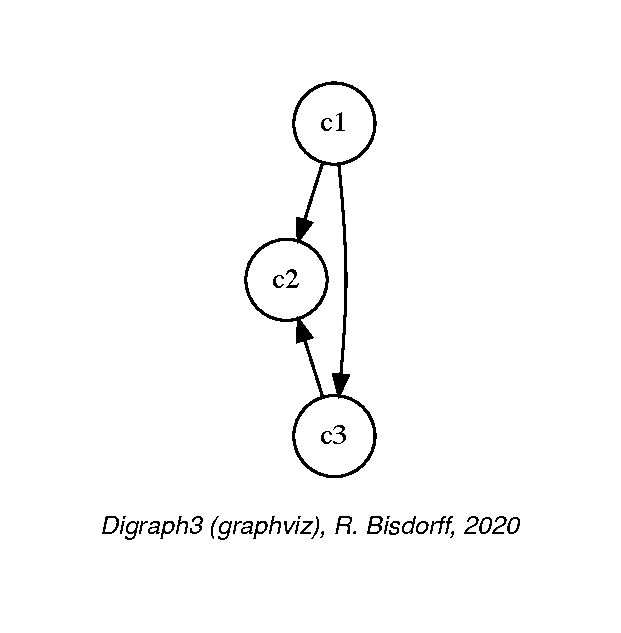
\includegraphics[width=5cm]{Figures/7-1-tutorialBallots.pdf}
\caption[Visualising an election result]{\emph{Visualising an election result}\\ In the Figure we notice that the \emph{majority margins} digraph from our example linear voting profile models in fact a linear ranking of the candidates: \texttt{c1} $>$ \texttt{c3} $>$ \texttt{c2}, the same actually as modelled by the \Borda scores (see List.~\vref{list:7.4}).}
\label{fig:7.1}       % Give a unique label
\end{figure}

That a majority margins digraph models a linear ranking of the eligible candidates, as shown in Fig.~\vref{fig:7.1}, represents a very unlikely event. Usually, when aggregating linear ballots, there appear cyclic social preferences.

\section{Cyclic social preferences}
\label{sec:7.4}

Let us consider for instance in Listing~\vref{list:7.7} the following linear voting profile \texttt{v} and construct the corresponding majority margins digraph.
\begin{lstlisting}[caption={Example of cyclic social preferences},label=list:7.7]
>>> v.showLinearBallots()
   voters(weight): candidates rankings
    v1(1): ['c1', 'c3', 'c5', 'c2', 'c4']
    v2(1): ['c1', 'c2', 'c4', 'c3', 'c5']
    v3(1): ['c5', 'c2', 'c4', 'c3', 'c1']
    v4(1): ['c3', 'c4', 'c1', 'c5', 'c2']
    v5(1): ['c4', 'c2', 'c3', 'c5', 'c1']
    v6(1): ['c2', 'c4', 'c5', 'c1', 'c3']
    v7(1): ['c5', 'c4', 'c3', 'c1', 'c2']
    v8(1): ['c2', 'c4', 'c5', 'c1', 'c3']
    v9(1): ['c5', 'c3', 'c4', 'c1', 'c2']
>>> mmdg = MajorityMarginsDigraph(v)
>>> mmdg.showRelationTable(ReflexiveTerms=False)
  * ---- Relation Table -----*
    M(x,y) | 'c1'  'c2'  'c3'  'c4'  'c5'	  
    -------|-----------------------------
     'c1'  |   -     1    -1    -5    -3  §\label{line:7.7.17}§
     'c2'  |  -1     - 	   1     1    -1	 
     'c3'  |   1    -1 	   -    -3    -1	 
     'c4'  |   5    -1     3     -     1  
     'c5'  |   3     1 	   1    -1     -  §\label{line:7.7.21}§ 
    Valuation domain: [-9;+9]
\end{lstlisting}    

Now there doesn't exist anymore a completely positive row in the relation table (see Lines~\ref{line:7.7.17}-\ref{line:7.7.21} in List.~\ref{list:7.7}). No one of the five candidates is beating all the others with an absolute majority of votes. There is no \Condorcet winner anymore. In fact, when looking in Fig.~\vref{fig:7.2} at a \texttt{graphviz} drawing of this \emph{majority margins} digraph, we may observe \emph{cyclic} voters's preferences, like \texttt{c1} $>$ \texttt{c2} $>$ \texttt{c3} $>$ \texttt{c1}.
\begin{lstlisting}
>>> mmdg.exportGraphViz('cycles',graphType='pdf')
 *---- exporting a dot file for GraphViz tools ----*
  Exporting to cycles.dot
  dot -Grankdir=BT -Tpng cycles.dot -o cycles.pdf
\end{lstlisting}
\begin{figure}[ht]
\sidecaption[t]
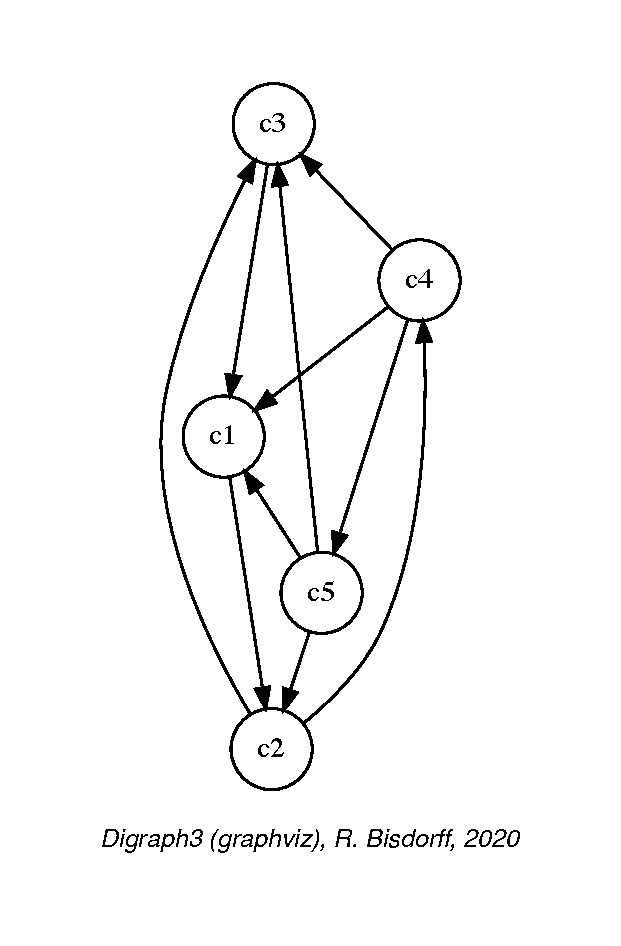
\includegraphics[width=5cm]{Figures/7-2-cycles.pdf}
\caption[Cyclic social preferences]{\emph{Cyclic social preferences}\\ \texttt{c1} $>$ \texttt{c2} $>$ \texttt{c3} $>$ \texttt{c1} for instance.}
\label{fig:7.2}       % Give a unique label
\end{figure}
	   
There may be many circuits appearing in a \emph{majority margins} digraph. The \texttt{computeChordlessCircuits} method\index{computeChordlessCircuits@\texttt{computeChordlessCircuits()}} detects and enumerates all minimal chordless circuits in a \texttt{Digraph} instance. 
\begin{lstlisting}
>>> mmdg.computeChordlessCircuits()
 [(['c2', 'c3', 'c1'], frozenset({'c2', 'c3', 'c1'})), 
  (['c2', 'c4', 'c5'], frozenset({'c2', 'c5', 'c4'})), 
  (['c2', 'c4', 'c1'], frozenset({'c2', 'c1', 'c4'}))]
\end{lstlisting}

In our example voting profile \texttt{v}, we actually obtain three chordless social preference circuits and determining the winner of this election result becomes non trivial. There is, for instance, no more any instant runoff winner.
\begin{lstlisting}
>>> v.computeInstantRunoffWinner(Comments=True)
Total number of votes =  9.000
Half of the Votes =  4.50
 ==> stage =  1
    remaining candidates ['c2', 'c5', 'c1', 'c4', 'c3']
    uninominal votes {'c2': 2.0, 'c5': 3.0, 'c1': 2.0, 'c4': 1.0, 'c3': 1.0}
    minimal number of votes =  1.0
    maximal number of votes =  3.0
    candidate to remove =  c3
    candidate to remove =  c4
    remaining candidates =  ['c2', 'c5', 'c1']
 ==> stage =  2
    remaining candidates ['c2', 'c5', 'c1']
    uninominal votes {'c2': 3.0, 'c5': 3.0, 'c1': 3.0}
    minimal number of votes =  3.0
    maximal number of votes =  3.0
    candidate to remove =  c1
    candidate to remove =  c5
    candidate to remove =  c2
    remaining candidates =  []
[]
\end{lstlisting}

\Condorcet 's approach for determining the winner of an election is \emph{not decisive} in this example voting profile. One needs therefore, the case given, exploiting more sophisticated approaches for finding the winner of the election on the basis of the given linear ballots (see Chap.~\ref{sec:8} and \citealp{BIS-2008a}). 

The \NetFlows ranked heatmap view on voting profiles\index{showHTMLVotingHeatmap@\texttt{showHTMLVotingHeatmap()}} with the \texttt{showHTML\-VotingHeatmap()} method is one such tool for showing convincing voting results (see Sect.~\ref{sec:8.3}).
\begin{lstlisting}[caption={\NetFlows ranked heatmap view on a voting profile},label=list:7.8]
>>> v.showHTMLVotingHeatmap(rankingRule='Netflows',\
...                  colorLevels=3,Correlations=True)
\end{lstlisting}
\begin{figure}[ht]
\sidecaption[t]
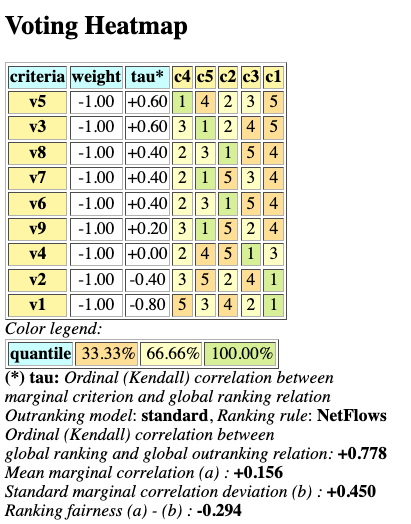
\includegraphics[width=7cm]{Figures/7-3-votingHeatmap.png}
\caption[Visualising a linear voting profile in a \NetFlows ranked heatmap]{\emph{Visualising a linear voting profile in a \NetFlows ranked heatmap}\\ As the number of voters is usually much larger than the number of eligible candidates, the voting heatmap is by default transposed into a voters $\times$ candidates view. Notice that the importance weights of the voters are \emph{negative}, which means that the preference direction of the criteria (in this case the individual voters) is \emph{decreasing} (\texttt{min}), i.e. goes from lowest (best) rank to highest (worst) rank.}
\label{fig:7.3}       % Give a unique label
\end{figure}

It is worthwhile noticing in Fig.~\vref{fig:7.3} that the compromise \NetFlows ranking \texttt{c4} $>$ \texttt{c5} $>$ \texttt{c2} $>$ \texttt{c3} $>$ \texttt{c1}, shown in this heatmap, results in the highest possible \emph{ordinal correlation} index of $+0.778$ with the majority margins digraph (see Chap.~\ref{sec:16}). This \NetFlows ranking result corresponds also to the \Borda scores ranking\footnote{Mind that \Borda scores require the unrealistic working hypothesis that one knows how to precisely code in numbers the marginal linear ranks per voter.}.
\begin{lstlisting}[caption={Rank analysis table with \Borda scores},label=list:7.9]
>>> v.showRankAnalysisTable()
  *----  Borda rank analysis tableau -----*
   candi- | alternative-to-rank       |      Borda
   dates  |  1    2    3    4    5    | score  average
   -------|-------------------------------------------------
     'c4' |  1    4    3    0    1    |  23     2.56
     'c5' |  3    0    3    2    1    |  25     2.78
     'c2' |  2    3    0    1    3    |  27     3.00
     'c3' |  1    2    2    2    2    |  29     3.22
     'c1' |  2    0    1    4    2    |  31     3.44
\end{lstlisting}

Let us eventually notice in the rank analysis table, shown in Listing~\ref{list:7.9} above, that the uninominal plurality winner would be, with three votes, candidate \texttt{c5}, whereas the best \NetFlows and \Borda ranked candidate \texttt{c1} obtains with candidate \texttt{c3} only one vote.

But do represent our example linear voting profiles here realistic election outcomes?

\section{On generating realistic random linear voting profiles}
\label{sec:7.5}

By default, the \texttt{RandomLinearVotingProfile} class generates random linear voting profiles where every candidate has the same uniform probability to be ranked at a certain position by all the voters. Each voter's random linear ballot is indeed generated  via a uniform shuffling of the list of candidates.

In reality, political election data are quite different. There usually will be different favorite and marginal candidates for each political party. To simulate these aspects with our random generator, we are using two random exponentially distributed polls of the candidates and consider a bipartisan political landscape with a certain random balance (default theoretical party repartition = $0.50$) between the two sets of potential party supporters. A certain theoretical proportion (default = $0.1$) will not support any party.

Let us generate in Listing~\vref{list:7.10} such a linear voting profile for an election with $1000$ voters and $15$ candidates.
\begin{lstlisting}[caption={Generating a linear voting profile with random polls},label=list:7.10]
>>> from votingProfiles import\
...            RandomLinearVotingProfile
>>> lvp = RandomLinearVotingProfile(\
...         numberOfCandidates=15,\
...         numberOfVoters=1000,\
...         WithPolls=True,\
...         partyRepartition=0.5,\
...         other=0.1,\
...         seed=0.9189670954954139)
>>> lvp
 *------- VotingProfile instance description ------*
  Instance class : RandomLinearVotingProfile
  Instance name  : randLinearProfile
  Candidates     : 15
  Voters         : 1000
  Attributes     : ['name', 'seed', 'candidates',
                    'voters', 'RandomWeights',
                    'sumWeights', 'poll1', 'poll2',
                    'bipartisan', 'linearBallot',
                    'ballot']
>>> lvp.showRandomPolls()   §\label{line:7.10.21}§ 
  Random repartition of voters
   Party-1 supporters : 460 (46.0%)
   Party-2 supporters : 436 (43.6%)
   Other voters       : 104 (10.4%)
  *---------------- random polls ----------------*
   Party-1(46.0%) | Party-2(43.6%)|  expected  
  ----------------------------------------------
   c06 : 19.91%  |  c11 : 22.94%  |  c06 : 15.00% §\label{line:7.10.29}§
   c07 : 14.27%  |  c08 : 15.65%  |  c11 : 13.08%
   c03 : 10.02%  |  c04 : 15.07%  |  c08 : 09.01%
   c13 : 08.39%  |  c06 : 13.40%  |  c07 : 08.79%
   c15 : 08.39%  |  c03 : 06.49%  |  c03 : 07.44%
   c11 : 06.70%  |  c09 : 05.63%  |  c04 : 07.11%
   c01 : 06.17%  |  c07 : 05.10%  |  c01 : 05.06%
   c12 : 04.81%  |  c01 : 05.09%  |  c13 : 05.04%
   c08 : 04.75%  |  c12 : 03.43%  |  c15 : 04.23%
   c10 : 04.66%  |  c13 : 02.71%  |  c12 : 03.71%
   c14 : 04.42%  |  c14 : 02.70%  |  c14 : 03.21%
   c05 : 04.01%  |  c15 : 00.86%  |  c09 : 03.10%
   c09 : 01.40%  |  c10 : 00.44%  |  c10 : 02.34%
   c04 : 01.18%  |  c05 : 00.29%  |  c05 : 01.97%
   c02 : 00.90%  |  c02 : 00.21%  |  c02 : 00.51% §\label{line:7.10.43}§ 
\end{lstlisting}

In this example (see above Lines~\ref{line:7.10.21} and following), we obtain 460 Party-1 supporters ($46\%$), 436 Party-2 supporters ($43.6\%$) and 104 other voters ($10.4\%$). Favorite candidates of Party-1 supporters, with more than $10\%$, appear to be \texttt{c06} ($19.91\%$), $c07$ ($14.27\%$) and \texttt{c03} ($10.02\%$). Whereas for Party-2 supporters, favorite candidates appear to be \texttt{c11} ($22.94\%$), followed by \texttt{c08} ($15.65\%$), $c04$ ($15.07\%$) and \texttt{c06} ($13.4\%$). Being \emph{first} choice for Party-1 supporters and \emph{fourth} choice for Party-2 supporters, this candidate \texttt{c06} is a natural candidate for clearly winning this election game (see List.~\vref{list:7.11}).
\begin{lstlisting}[caption={The uninominal and \Borda election winner},label=list:7.11]
>>> lvp.computeSimpleMajorityWinner()
 ['c06']
>>> lvp.computeInstantRunoffWinner()
 ['c06']  
>>> lvp.computeBordaWinners()
 ['c06']
\end{lstlisting}

Is candidate \texttt{c06} also a \Condorcet winner? To verify, we start by creating the corresponding \emph{majority margins} digraph $mmdg$ with the help of the \texttt{MajorityMarginsDi\-graph} class. The created digraph instance contains 15 \emph{actions} --the candidates-- and 104 \emph{oriented arcs} --the \emph{positive} majority margins-- (see List.~\vref{list:7.12} Lines~\ref{line:7.12.7}-\ref{line:7.12.8}).
\begin{lstlisting}[caption={A majority margins digraph constructed from a linear voting profile},label=list:7.12]
>>> from votingProfiles import MajorityMarginsDigraph
>>> mmdg = MajorityMarginsDigraph(lvp)
>>> mmdg
 *------- Digraph instance description ------*
  Instance class      : MajorityMarginsDigraph
  Instance name       : rel_randLinearProfile
  Digraph Order       : 15 §\label{line:7.12.7}§ 
  Digraph Size        : 104 §\label{line:7.12.8}§ 
  Valuation domain    : [-1000.00;1000.00]
  Determinateness (%) : 67.08
  Attributes          : ['name', 'actions', 'voters',
                         'ballot', 'valuationdomain',
                         'relation', 'order',
                         'gamma', 'notGamma']
\end{lstlisting}

The \texttt{showHTMLRelationTable()} method visualise the resulting pairwise majority margins by showing the HTML formated version of the \texttt{mmdg} relation table in a browser view.\index{showHTMLRelationTable@\texttt{showHTMLRelationTable()}}
\begin{lstlisting}
>>> mmdg.showHTMLRelationTable(\
...         tableTitle='Pairwise majority margins',
...         relationName='M(x,y)')
\end{lstlisting}
\begin{figure}[ht]
\sidecaption[t]
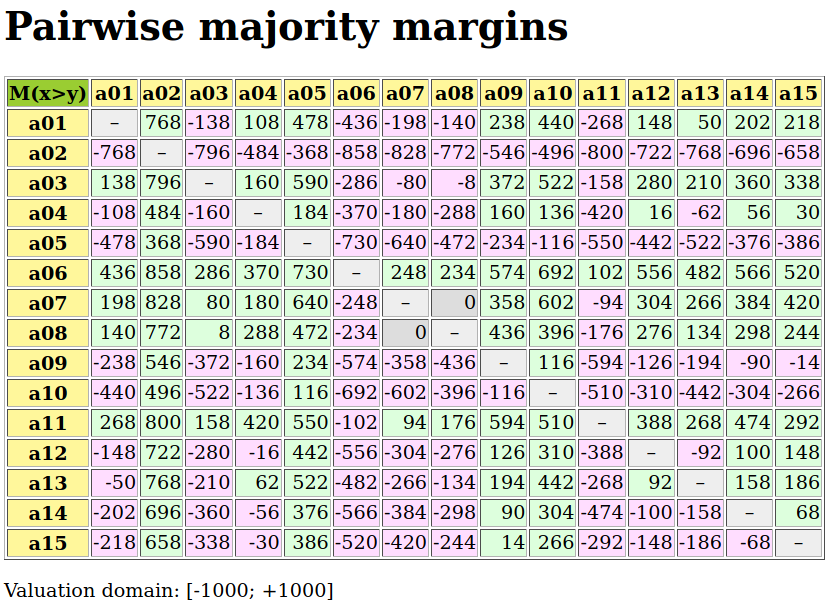
\includegraphics[width=7cm]{Figures/7-4-majorityMargins.png}
\caption[Browsing the majority margins]{\emph{Browsing the majority margins}\\ \emph{Light green} cells contain the positive majority margins, whereas \emph{light red} cells contain the negative majority margins.}
\label{fig:7.4}       % Give a unique label
\end{figure}

A complete light green \emph{row} in Fig.~\vref{fig:7.4} reveals a \Condorcet winner, whereas a complete light green \emph{column} reveals a \Condorcet loser. We recover again candidate \texttt{c06} as \Condorcet winner\footnote{The concept of \Condorcet winner --a generalisation of absolute majority winners-- proposed by \Condorcet in 1784, is an early historical example of initial digraph kernel (see Chap.~\ref{sec:17}).}, whereas the obvious \Condorcet loser is here candidate \texttt{c02}, the candidate with the lowest support in both parties (see List.~\vref{list:7.10} Line~\ref{line:7.10.43}).

With a same bipolar \emph{first-ranked} and \emph{last-ranked} selection procedure\index{computeRankingByChoosing@\texttt{computeRankingByChoosing()}}, we may weakly rank the candidates (with possible ties) by iterating these \emph{first-ranked} and \emph{last-ranked} choices among the remaining candidates \citep{BIS-1999}.

Before showing the \emph{ranking-by-choosing} result, we have to, first, compute the iterated bipolar selection procedure (see List.~\vref{list:7.13}).\index{showRankingByChoosing@\texttt{showRankingByChoosing()}}
\begin{lstlisting}[caption={Ranking by iterating choosing the \emph{first} and \emph{last} remaining candidates },label=list:7.13]
>>> cdg.showRankingByChoosing()
 Ranking by Choosing and Rejecting
   1st best ranked ['c06']
     2nd best ranked ['c11']
       3rd  best ranked ['c07','c08']  §\label{line:7.13.5}§
         4th best ranked ['c03']
           5th best ranked ['c01']
             6th best ranked ['c13']
               7th first ranked ['c04']   §\label{line:7.13.9}§ 
               7th last ranked ['c12']    §\label{line:7.13.10}§ 
	     6th last ranked ['c14']
	   5th last ranked ['c15']
	 4th last ranked ['c09']
       3rd last ranked ['c10']
     2nd last ranked ['c05']
   1st last ranked ['c02']
\end{lstlisting}

The first selection concerns \texttt{c06} (first) and \texttt{c02} (last), followed by \texttt{c11} (first) opposed to \texttt{c05} (last), and so on, until there remains at iteration step 7 a last pair of candidates, namely [\texttt{c04}, \texttt{c12}] (see Lines~\ref{line:7.13.9}-\ref{line:7.13.10}).

Notice furthermore the 3rd-best ranked candidates at iteration step 3 (see Line~\ref{line:7.13.5}), namely the pair (\texttt{c07}, \texttt{c08}). Both candidates represent indeed conjointly the \emph{3rd best ranked} choice. We obtain hence a \emph{weak ranking}, i.e. a ranking with a tie.

Let us mention that the \emph{instant runoff} procedure, we used before when operated with a \texttt{Comments=True} parameter setting, will deliver a more or less similar \emph{reversed} linear \emph{ordering-by-rejecting} result, namely \texttt{[c02, c10, c14, c05, c09, c13, c12, c15, c04, c01, c08, c03, c07, c11, c06]}, ordered from the \emph{last} to the \emph{first} choice.

Remarkable about both these \emph{ranking-by-choosing} or \emph{ordering-by-rejecting} results is the fact that the random voting behaviour, simulated here with the help of two discrete random variables \footnote{Discrete random variables with a given empirical probability law (here the polls) are provided in the \texttt{randomNumbers} module by the \texttt{DiscreteRandomVariable} class \citep{CPSTAT-L4}.}, defined respectively by the two random party polls, is rendering a ranking that is more or less in accordance with the simulated balance of the polls: Party-1 supporters : 460;  Party-2 supporters: 436 (see List.~\vref{list:7.10} Lines~\ref{line:7.10.29}-\ref{line:7.10.43} third column). Despite a random voting behaviour per voter, the given polls apparently show a \emph{very strong incidence} on the eventual election result. In order to avoid any manipulation of the election outcome, public media are therefore in some countries not allowed to publish polls during the last weeks before a general election.

Mind that the specific \emph{ranking-by-choosing} procedure, we use here on the majority margins digraph, operates the selection procedure by extracting at each step \emph{initial} and \emph{terminal} prekernels, i.e. difficult operational problems (see Chap.~\ref{sec:17} and \citealp{BIS-1999}); A technique that does not allow in general to tackle voting profiles with much more than 30 candidates.

\vspace{\baselineskip}

Next Chap.~\ref{sec:8} on multiple incommensurable criteria ranking methods presents more methods and tools for ranking from pairwise majority margins when a larger number of potential candidates or decision alternatives is given.  

%%%%%%% The chapter bibliography
%\normallatexbib
%\clearpage
%\phantomsection
%\addcontentsline{toc}{section}{Chapter Bibliography}
\chapter{Computing the winner of an election}
\label{sec:7}

\abstract*{To be written.}
  
\abstract{To be written.}

\section{Linear voting profiles}
\label{sec:7.1}

The {\tt votingProfiles}\index{votingProfiles@\texttt{votingProfiles} module} module provides resources for handling election results \citep{ADT-L2}, like the \texttt{LinearVotingProfile} class\index{LinearVotingProfile@\texttt{LinearVotingProfile} class}. We consider an election involving a finite set of candidates and finite set of weighted voters, who express their voting preferences in a complete linear ranking (without ties) of the candidates. The data is internally stored in two ordered dictionaries, one for the voters and another one for the candidates. The linear ballots are stored in a standard dictionary.
\begin{lstlisting}
candidates = OrderedDict([
  ('a1',...), ('a2',...), ('a3', ...), ...}
voters = OrderedDict([
  ('v1',{'weight':10}),
  ('v2',{'weight':3}),
  ... ])
  # each voter specifies a
  # linearly ranked list of candidates
  # from the best to the worst (without ties
linearBallot = {
  'v1' : ['a2','a3','a1', ...],
  'v2' : ['a1','a2','a3', ...],
   ...
  }
\end{lstlisting}

The module provides a \texttt{RandomLinearVotingProfile} class \index{RandomLinearVotingProfile@\texttt{RandomLinearVotingProfile} class} for generating random instances of the \texttt{LinearVotingProfile} class. In an interactive Python session we may obtain for the election of 3 candidates by 5 voters the following result.
\begin{lstlisting}[caption={Example of random linear voting profile},label=list:7.1]
>>> from votingProfiles import\
...              RandomLinearVotingProfile
>>> lvp = RandomLinearVotingProfile(numberOfVoters=5,\
...                               numberOfCandidates=3,\
...                               RandomWeights=True) 
>>> lvp.candidates
  OrderedDict([ ('a1',{'name':'a1}),
                ('a2',{'name':'a2'}),
                ('a3',{'name':'a3'}) ])
>>> lvp.voters
  OrderedDict([('v1',{'weight': 2}),
               ('v2':{'weight': 3}), 
               ('v3',{'weight': 1}),
               ('v4':{'weight': 5}),
               ('v5',{'weight': 4})])
>>> lvp.linearBallot
    {'v1': ['a1', 'a2', 'a3',],
     'v2': ['a3', 'a2', 'a1',],
     'v3': ['a1', 'a3', 'a2',],
     'v4': ['a1', 'a3', 'a2',],
     'v5': ['a2', 'a3', 'a1',]} 
 \end{lstlisting}

Notice that in this random example, the five voters are weighted (see Listing \ref{list:7.1} Line 6-7). Their linear ballots can be viewed with the \texttt{showLinearBallots}\index{()showLinearBallots@\texttt{showLinearBallots}} method.
\begin{lstlisting}
>>> lvp.showLinearBallots()
    voters(weight)	 candidates rankings
    v1(2): 	 ['a2', 'a1', 'a3']
    v2(3): 	 ['a3', 'a1', 'a2']
    v3(1): 	 ['a1', 'a3', 'a2']
    v4(5): 	 ['a1', 'a2', 'a3']
    v5(4): 	 ['a3', 'a1', 'a2']
    nbr. of voters: 15
\end{lstlisting}

Editing of the linear voting profile may be achieved by storing the data in a file, edit it, and reload it again.
\begin{lstlisting}
>>> v.save(fileName='tutorialLinearVotingProfile1')
   *--- Saving linear profile in file:
                   <tutorialLinearVotingProfile1.py> ---*
>>> from votingProfiles import LinearVotingProfile
>>> v = LinearVotingProfile('tutorialLinearVotingProfile1')
\end{lstlisting}

\section{Computing the winner}
\label{sec:7.2}

We may easily compute \emph{uninominal votes}\index{uninominal votes}, i.e. how many times a candidate was ranked first, and see who is consequently the \emph{simple majority} (plurality) winner(s) in this election.
\begin{lstlisting}
>>> v.computeUninominalVotes()
  {'a2': 2, 'a1': 6, 'a3': 7}
>>> v.computeSimpleMajorityWinner()
  ['a3']
\end{lstlisting}

As we observe no absolute majority (8/15) of votes for any of the three candidate, we may look for the \emph{instant runoff} winner\index{computeInstantRunoffWinner@\texttt{computeInstantRunoffWinner()}} instead (see \citet{ADT-L2}).
\begin{lstlisting}[caption={Example Instant Run Off Winner},label=list:7.2]
>>> v.computeInstantRunoffWinner(Comments=True)
  Half of the Votes =  7.50
    ==> stage =  1
	remaining candidates ['a1', 'a2', 'a3']
	uninominal votes {'a1': 6, 'a2': 2, 'a3': 7}
	minimal number of votes =  2
	maximal number of votes =  7
	candidate to remove =  a2
	remaining candidates =  ['a1', 'a3']
    ==> stage =  2
	remaining candidates ['a1', 'a3']
	uninominal votes {'a1': 8, 'a3': 7}
	minimal number of votes =  7
	maximal number of votes =  8
	candidate a1 obtains an absolute majority
   Instant run off winner: ['a1']
 \end{lstlisting}
In stage 1, no candidate obtains an absolute majority of votes. Candidate \texttt{a2} obtains the minimal number of votes (2/15) and is, hence, eliminated. In stage 2, candidate \texttt{a1} obtains an absolute majority of the votes (8/15) and is eventually elected (see Listing \ref{list:7.2}).

We may also follow the \emph{Chevalier de Borda}'s advice and, after a \textbf{rank analysis} of the linear ballots, compute the \emph{Borda score} -the average rank- of each candidate and hence determine the \emph{Borda winner(s)}\index{computeRankAnalysis@\texttt{computeRankAnalysis()}}.
\begin{lstlisting}[caption={Example of \emph{Borda} rank scores},label=list:7.3]
>>> v.computeRankAnalysis()
 {'a2': [2, 5, 8], 'a1': [6, 9, 0], 'a3': [7, 1, 7]}
>>> v.computeBordaScores()
 OrderedDict([
   ('a1', {'BordaScore': 24, 'averageBordaScore': 1.6}),
   ('a3', {'BordaScore': 30, 'averageBordaScore': 2.0}),
   ('a2', {'BordaScore': 36, 'averageBordaScore': 2.4}) ])
>>> v.computeBordaWinners()
 ['a1']
\end{lstlisting}
Candidate \texttt{a1} obtains the minimal \emph{Borda} score, followed by candidate \texttt{a3} and finally candidate \texttt{a2} (see Listing \ref{list:7.3}). The corresponding \emph{Borda rank analysis table} may be printed out with a corresponding \texttt{showRankAnalysisTable()} command \index{showRankAnalysisTable@\texttt{showRankAnalysisTable()}}.
\begin{lstlisting}[caption={Rank analysis example},label=list:7.4]
>>> v.showRankAnalysisTable()
 *----  Borda rank analysis tableau -----*
  candi- | alternative-to-rank |     Borda
  dates  |   1     2     3     | score  average
  -------|-------------------------------------
   'a1'  |   6     9     0     | 24/15   1.60
   'a3'  |   7     1     7     | 30/15   2.00
   'a2'  |   2     5     8     | 36/15   2.40
 \end{lstlisting}

In our randomly generated election results, we are lucky: The instant runoff winner and the \emph{Borda} winner both is candidate \texttt{a1} (see Listings \ref{list:7.2} and \ref{list:7.3}). However, we could also follow the \emph{Marquis de Condorcet}'s advice, and compute the \emph{majority margins} obtained by voting for each individual pair of candidates.

\section{The majority margins digraph}
\label{sec:7.3}

For instance, candidate \texttt{a1} is ranked four times before and once behind candidate \texttt{a2}. Hence the corresponding \emph{majority margin}\index{majority margins} $M(a_1,a_2)$ is $4 - 1 = +3$. These \emph{majority margins} define on the set of candidates what we call the \emph{majority margins digraph}\index{majority margins digraph}. The \texttt{MajorityMarginsDigraph} class\index{MajorityMarginsDigraph@\texttt{MajorityMarginsDigraph} class} (a specialization of the root \texttt{Digraph} class) is available for handling such kind of digraphs.
\begin{lstlisting}[caption={Example of \emph{Majority Margins} digraph},label=list:7.5]
>>> from votingProfiles import MajorityMarginsDigraph
>>> mmdg = MajorityMarginsDigraph(lvp,\
...                IntegerValuation=True)
>>> mmdg
 *------- Digraph instance description ------*
  Instance class      : MajorityMarginsDigraph
  Instance name       : rel_randomLinearVotingProfile1
  Digraph Order       : 3
  Digraph Size        : 3
  Valuation domain    : [-15.00;15.00]
  Determinateness (%) : 64.44
  Attributes          : ['name', 'actions', 'voters',
                         'ballot', 'valuationdomain',
                         'relation', 'order',
                         'gamma', 'notGamma']
>>> mmdg.showAll()
 *----- show detail -------------*
  Digraph          : rel_randLinearVotingProfile1
  *---- Actions ----*
   ['a1', 'a2', 'a3']
  *---- Characteristic valuation domain ----*
  {'max': Decimal('15.0'),
   'med': Decimal('0'),
   'min': Decimal('-15.0'),
   'hasIntegerValuation': True}
  *---- majority margins -----*
     M(x,y) |  'a1'   'a2'  'a3'	  
    --------|-------------------
      'a1'  |    0     11     1	 
      'a2'  |  -11      0    -1	 
      'a3'  |   -1      1     0	 
    Valuation domain: [-15;+15]
\end{lstlisting}

Notice that, in the case of linear voting profiles, majority margins always verify a \emph{zero sum property}: $M(x,y) + M(y,x) = 0$ for all candidates $x$ and $y$ (see Listing \ref{list:7.5} Lines 26-28). This is not true in general for arbitrary voting profiles. The \emph{majority margins} digraph of linear voting profiles defines in fact a \emph{weak tournament}\index{weak tournament} and belongs, hence, to the class of \emph{self-codual} bipolar-valued digraphs\footnote{The class of self-codual bipolar-valued digraphs consists of all weakly asymmetric digraphs, i.e. digraphs containing only asymmetric and/or indeterminate links. Limit cases consists of, on the one side, full tournaments with indeterminate reflexive links, and, on the other side, fully indeterminate digraphs. In this class, the converse (inverse $\sim$) operator is indeed identical to the dual (negation $-$ ) one.}.
    
Now, a candidate $x$, showing a positive majority margin $M(x,y)$, is beating candidate $y$  with an absolute majority in a pairwise voting. Hence, a candidate showing only positive terms in her row in the \emph{majority margins} digraph relation table, beats all other candidates with absolute majority of votes. \Condorcet recommends to declare this candidate (is always unique, why?) the winner of the election. Here we are lucky, it is again candidate \texttt{a1} who is hence the \emph{Condorcet winner}\index{Condorcet!winner} (see Listing \ref{list:7.5} Line 26).
\begin{lstlisting}
>>> mmdg.computeCondorcetWinners()
 ['a1']  
\end{lstlisting}    

By seeing the majority margins like a \emph{bipolar-valued characteristic function} of a global preference relation defined on the set of candidates, we may use all operational resources of the generic \texttt{Digraph} class (see Chapter \ref{sec:2}), and especially its \texttt{exportGraphViz()} method \footnote{The \texttt{exportGraphViz()} method is depending on drawing tools from the graphviz software (https://graphviz.org/).}, for visualizing an election result.
\begin{lstlisting}
>>> mmdg.exportGraphViz(fileName='tutorialLinearBallots')
 *---- exporting a dot file for GraphViz tools ---------*
  Exporting to tutorialLinearBallots.dot
  dot -Grankdir=BT -Tpng tutorialLinearBallots.dot \
                   -o tutorialLinearBallots.png
\end{lstlisting}
\begin{figure}[h]
\sidecaption[t]
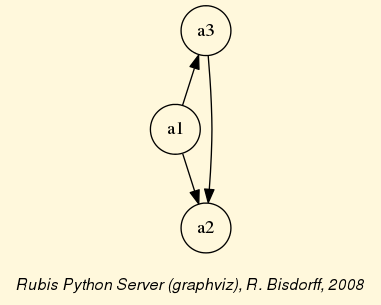
\includegraphics[width=6cm]{Figures/tutorialLinearBallots.png}
\caption{Visualizing an election result. In the Figure we notice that the \emph{majority margins} digraph from our example linear voting profile gives a linear order of the candidates: $a_1 > a_3 > a_2$, the same actually as given by the \emph{Borda} scores (see Listing \ref{list:7.4}). This is by far not given in general. Usually, when aggregating linear ballots, there appear cyclic social preferences.
}
\label{fig:7.1}       % Give a unique label
\end{figure}

\section{Cyclic social preferences}
\label{sec:7.4}

Let us consider for instance the following linear voting profile $v$ and construct the corresponding majority margins digraph.
\begin{lstlisting}[caption={Example of cyclic social preferences},label=list:7.6]
>>> v.showLinearBallots()
   voters(weight): candidates rankings
    v1(1): ['a1', 'a3', 'a5', 'a2', 'a4']
    v2(1): ['a1', 'a2', 'a4', 'a3', 'a5']
    v3(1): ['a5', 'a2', 'a4', 'a3', 'a1']
    v4(1): ['a3', 'a4', 'a1', 'a5', 'a2']
    v5(1): ['a4', 'a2', 'a3', 'a5', 'a1']
    v6(1): ['a2', 'a4', 'a5', 'a1', 'a3']
    v7(1): ['a5', 'a4', 'a3', 'a1', 'a2']
    v8(1): ['a2', 'a4', 'a5', 'a1', 'a3']
    v9(1): ['a5', 'a3', 'a4', 'a1', 'a2']
>>> mmdg = MajorityMarginsDigraph(v)
>>> mmdg.showRelationTable()
    * ---- Relation Table -----
      S   |  'v1'   'v2'   'v3'	  'v4'	  'v5'	  
    ------|----------------------------------------
    'v1'  |   -     0.11  -0.11	 -0.56	 -0.33	 
    'v2'  | -0.11    -	   0.11	  0.11	 -0.11	 
    'v3'  |  0.11  -0.11    -	 -0.33	 -0.11	 
    'v4'  |  0.56  -0.11   0.33	   -	  0.11	 
    'v5'  |  0.33   0.11   0.11	 -0.11	   -	 
\end{lstlisting}    
Now, we cannot find any completely positive row in the relation table (see Listing \ref{list:7.6} Lines 17 - ). No one of the five candidates is beating all the others with an absolute majority of votes. There is no \emph{Condorcet} winner anymore. In fact, when looking at a graphviz drawing of this \emph{majority margins} digraph, we may observe \textbf{cyclic} preferences, like $(v_1 > v_2 > v_3 > v_1)$ for instance.
\begin{lstlisting}
>>> mmdg.exportGraphViz('cycles')
 *---- exporting a dot file for GraphViz tools ---------*
  Exporting to cycles.dot
  dot -Grankdir=BT -Tpng cycles.dot -o cycles.png
\end{lstlisting}
\begin{figure}[h]
\sidecaption[t]
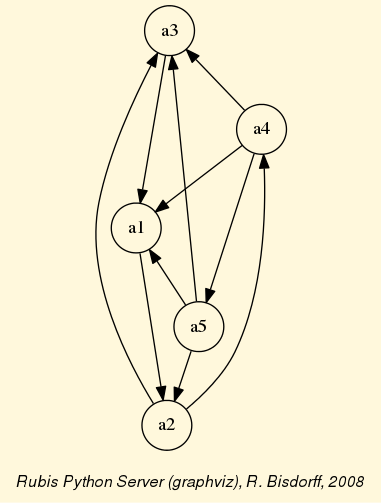
\includegraphics[width=4cm]{Figures/cycles.png}
\caption{Cyclic social preferences.}
\label{fig:7.2}       % Give a unique label
\end{figure}
	   
But, there may be many cycles appearing in a \emph{majority margins} digraph, and, we may detect and enumerate all minimal chordless circuits in a Digraph instance with the \texttt{computeChordlessCircuits} method.\index{computeChordlessCircuits}
\begin{lstlisting}
>>> mmdg.computeChordlessCircuits()
 [(['a2', 'a3', 'a1'], frozenset({'a2', 'a3', 'a1'})), 
  (['a2', 'a4', 'a5'], frozenset({'a2', 'a5', 'a4'})), 
  (['a2', 'a4', 'a1'], frozenset({'a2', 'a1', 'a4'}))]
\end{lstlisting}

\Condorcet 's approach for determining the winner of an election is hence \emph{not decisive} in all circumstances and we need to exploit more sophisticated approaches for finding the winner of the election on the basis of the majority margins of the given linear ballots (see Chapter ref{sec:8} and \citet{BIS-2008a}). 

Many more tools for exploiting voting results are available like the browser heat map view on voting profiles\index{showHTMLVotingHeatmap@\texttt{showHTMLVotingHeatmap()}}. The number of voters is usually much larger than the number of candidates. In that case, it is better to generate a transposed \emph{voters} $\times$ \emph{candidates} view (see Line 2 below) 
\begin{lstlisting}
>>> v.showHTMLVotingHeatmap(rankingRule='NetFlows',
...                         Transposed=False)
\end{lstlisting}
\begin{figure}[h]
\sidecaption[t]
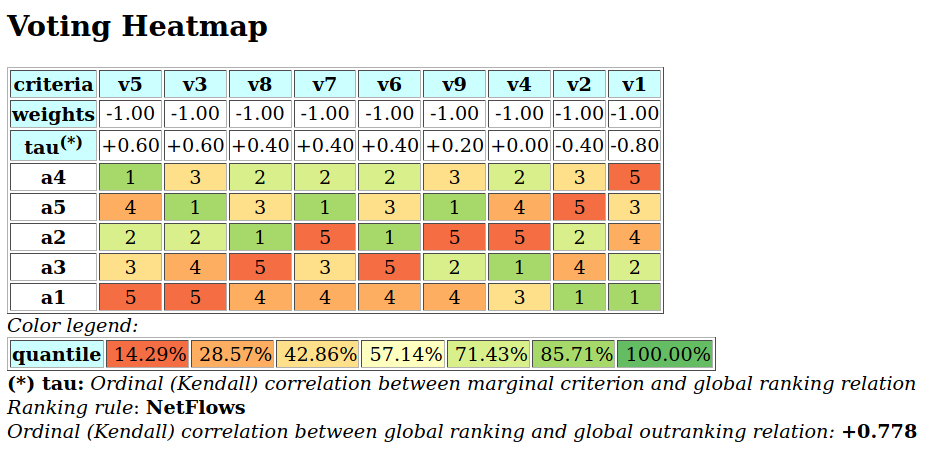
\includegraphics[width=4cm]{Figures/votingHeatmap.png}
\caption{Visualizing a linear voting profile in a heatmap format. Notice that the importance weights of the voters are \emph{negative}, which means that the preference direction of the criteria (in this case the individual voters) is \emph{decreasing}, i.e. goes from lowest (best) rank to highest (worst) rank.
}
\label{fig:7.3}       % Give a unique label
\end{figure}

It worthwhile noticing that the compromise \emph{NetFlows} ranking \texttt{a4} $>$ \texttt{a5} $>$ \texttt{a2} $>$ \texttt{a1} $>$ \texttt{a3}, shown in this heatmap (see Fig. \ref{fig:7.3}) results in an optimal \emph{ordinal correlation} index of $+0.778$ with the pairwise majority voting margins (see Chapter \ref{sec:16}). 

\section{On generating realistic random linear voting profiles}
\label{sec:7.5}

By default, the \texttt{RandomLinearVotingProfile} class generates random linear voting profiles where every candidates has the same uniform probabilities to be ranked at a certain position by all the voters. Each voter's random linear ballot is indeed generated  via a uniform shuffling of the list of candidates.

In reality, political election data appear quite different. There usually will be different favorite and marginal candidates for each political party. To simulate these aspects into our random generator, we are using two random exponentially distributed polls of the candidates and consider a bipartisan political landscape with a certain random balance (default theoretical party repartition = $0.50$) between the two sets of potential party supporters. A certain theoretical proportion (default = $0.1$) will not support any party.

Let us generate such a linear voting profile for an election with $1000$ voters and $15$ candidates.

\begin{lstlisting}[caption={Generating a linear voting profile with random polls},label=list:7.7]
>>> from votingProfiles import\
...            RandomLinearVotingProfile
>>> lvp = RandomLinearVotingProfile(\
...         numberOfCandidates=15,
...         numberOfVoters=1000,
...         WithPolls=True,
...         partyRepartition=0.5,
...         other=0.1,
...         seed=0.9189670954954139)
>>> lvp
 *------- VotingProfile instance description ------*
  Instance class : RandomLinearVotingProfile
  Instance name  : randLinearProfile
  Candidates     : 15
  Voters         : 1000
  Attributes     : ['name', 'seed', 'candidates',
                    'voters', 'RandomWeights',
                    'sumWeights', 'poll1', 'poll2',
                    'bipartisan', 'linearBallot',
                    'ballot']
>>> lvp.showRandomPolls()
  Random repartition of voters
   Party_1 supporters : 460 (46.0%)
   Party_2 supporters : 436 (43.6%)
   Other voters       : 104 (10.4%)
 *---------------- random polls ----------------*
   Party-1(46.0%) | Party-2(43.6%)|  expected  
  ----------------------------------------------
    a06 : 19.91%  | a11 : 22.94%  | a06 : 15.00%
    a07 : 14.27%  | a08 : 15.65%  | a11 : 13.08%
    a03 : 10.02%  | a04 : 15.07%  | a08 : 09.01%
    a13 : 08.39%  | a06 : 13.40%  | a07 : 08.79%
    a15 : 08.39%  | a03 : 06.49%  | a03 : 07.44%
    a11 : 06.70%  | a09 : 05.63%  | a04 : 07.11%
    a01 : 06.17%  | a07 : 05.10%  | a01 : 05.06%
    a12 : 04.81%  | a01 : 05.09%  | a13 : 05.04%
    a08 : 04.75%  | a12 : 03.43%  | a15 : 04.23%
    a10 : 04.66%  | a13 : 02.71%  | a12 : 03.71%
    a14 : 04.42%  | a14 : 02.70%  | a14 : 03.21%
    a05 : 04.01%  | a15 : 00.86%  | a09 : 03.10%
    a09 : 01.40%  | a10 : 00.44%  | a10 : 02.34%
    a04 : 01.18%  | a05 : 00.29%  | a05 : 01.97%
    a02 : 00.90%  | a02 : 00.21%  | a02 : 00.51%
\end{lstlisting}

In this example (see Listing \ref{list:7.7} Lines 18-), we obtain 460 Party-1 supporters ($46\%$), 436 Party-2 supporters ($43.6\%$) and 104 other voters ($10.4\%$). Favorite candidates of Party-1 supporters, with more than $10\%$, appear to be \texttt{a06} ($19.91\%$), $a07$ ($14.27\%$) and \texttt{a03} ($10.02\%$). Whereas for Party-2 supporters, favorite candidates appear to be \texttt{a11} ($22.94\%$), followed by \texttt{a08} ($15.65\%$), $a04$ ($15.07\%$) and \texttt{a06} ($13.4\%$). Being \emph{first} choice for Party-1 supporters and \emph{fourth} choice for Party-2 supporters, this candidate \texttt{a06} is a natural candidate for clearly winning this election game (see Listing \ref{list:7.8}).
\begin{lstlisting}[caption={The uninominal and \emph{Borda} election winner},label=list:7.8]
>>> lvp.computeSimpleMajorityWinner()
 ['a06']
>>> lvp.computeInstantRunoffWinner()
 ['a06']  
>>> lvp.computeBordaWinners()
 ['a06']
\end{lstlisting}

Is it also a \Condorcet winner ? To verify, we start by creating the corresponding \emph{majority margins} digraph $mmdg$ with the help of the \texttt{MajorityMarginsDigraph} class. The created digraph instance contains 15 \emph{actions} --the candidates-- and 105 \emph{oriented arcs} --the \emph{positive} majority margins-- (see Listing \ref{list:7.9} Lines 7-8).
\begin{lstlisting}[caption={A majority margins digraph constructed from a linear voting profile},label=list:7.9]
>>> from votingProfiles import MajorityMarginsDigraph
>>> mmdg = MajorityMarginsDigraph(lvp)
>>> mmdg
 *------- Digraph instance description ------*
  Instance class      : MajorityMarginsDigraph
  Instance name       : rel_randLinearProfile
  Digraph Order       : 15
  Digraph Size        : 104
  Valuation domain    : [-1000.00;1000.00]
  Determinateness (%) : 67.08
  Attributes          : ['name', 'actions', 'voters',
                         'ballot', 'valuationdomain',
                         'relation', 'order',
                         'gamma', 'notGamma']
\end{lstlisting}

We may visualize the resulting pairwise majority margins by showing the HTML formated version of the $mmdg$ relation table in a browser view.
\begin{lstlisting}
>>> cdg.showHTMLRelationTable(\
...         tableTitle='Pairwise majority margins',
...         relationName='M(x>y)')
\end{lstlisting}
\begin{figure}[h]
\sidecaption[t]
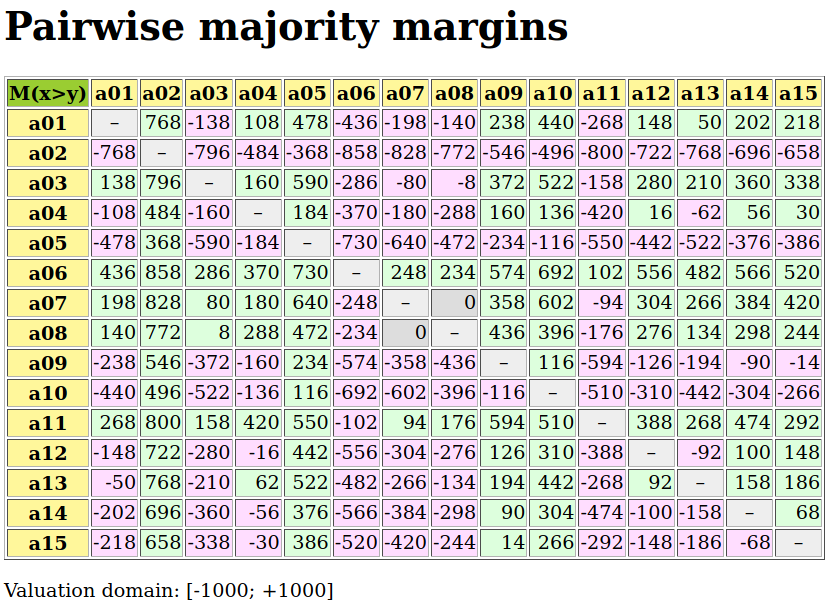
\includegraphics[width=4cm]{Figures/majorityMargins.png}
\caption{Browsing the majority margins. \emph{Light green} cells contain the positive majority margins, whereas \emph{light red} cells contain the negative majority margins.}
\label{fig:7.4}       % Give a unique label
\end{figure}

A complete \emph{light green} row reveals a \Condorcet winner, whereas a complete \emph{light green} column reveals a \Condorcet loser. We recover again candidate \texttt{a06} as \emph{Condorcet} winner\footnote{The concept of \Condorcet winner --a generalization of absolute majority winners-- proposed by \Condorcet in 1785, is an early historical example of initial digraph kernel (see Chapter \ref{sec:17})}.), whereas the obvious \emph{Condorcet} loser is here candidate \texttt{a02}, the candidate with the lowest support in both parties (see Listing \ref{list:7.7} Line 40).

With a same \emph{bipolar-first ranked} and \emph{last ranked} candidate- selection procedure\index{computeRankingByChoosing@\texttt{computeRankingByChoosing()}}, we may \emph{weakly rank} the candidates (with possible ties) by iterating these \emph{first ranked} and \emph{last ranked} choices among the remaining candidates \citep{BIS-1999}.

Before showing the \emph{ranking-by-choosing} result, we have to compute the iterated bipolar selection procedure (see Listing \ref{list:7.10} Line 2).
\begin{lstlisting}[caption={Ranking by iterating choosing the \emph{first} and \emph{last} remaining candidates },label=list:7.10]
>>> cdg.showRankingByChoosing()
 Error: You must first run
  self.computeRankingByChoosing(CoDual=False(default)|True) !
>>> cdg.computeRankingByChoosing()
>>> cdg.showRankingByChoosing()
 Ranking by Choosing and Rejecting
   1st first ranked ['a06']
     2nd first ranked ['a11']
       3rd first ranked ['a07', 'a08']
         4th first ranked ['a03']
           5th first ranked ['a01']
             6th first ranked ['a13']
               7th first ranked ['a04']
               7th last ranked ['a12']
	     6th last ranked ['a14']
	   5th last ranked ['a15']
	 4th last ranked ['a09']
       3rd last ranked ['a10']
     2nd last ranked ['a05']
   1st last ranked ['a02']
\end{lstlisting}
The first selection concerns \texttt{a06} (first) and \texttt{a02} (last), followed by \texttt{a11} (first) opposed to \texttt{a05} (last), and so on, until there remains at iteration step 7 a last pair of candidates, namely [\texttt{a04}, \texttt{a12}] (see Lines 13-14).

Notice furthermore the first ranked candidates at iteration step 3 (see Line 9), namely the pair (\texttt{a07}, \texttt{a08}). Both candidates represent indeed conjointly the \emph{first ranked} choice. We obtain here hence a \emph{weak ranking}, i.e. a ranking with a tie.

Let us mention that the \emph{instant-run-off} procedure, we used before (see Listing \ref{list:7.8} Line 3), when operated with a \texttt{Comments=True} parameter setting, will deliver a more or less similar \emph{reversed} linear \emph{ordering-by-rejecting} result, namely \texttt{[a02, a10, a14, a05, a09, a13, a12, a15, a04, a01, a08, a03, a07, a11, a06]}, ordered from the \emph{last} to the \emph{first} choice.

Remarkable about both these \emph{ranking-by-choosing} or \emph{ordering-by-rejecting} results is the fact that the random voting behaviour, simulated here with the help of two discrete random variables \footnote{Discrete random variables with a given empirical probability law (here the polls) are provided in the \texttt{randomNumbers} module by the \texttt{DiscreteRandomVariable} class.}, defined respectively by the two party polls, is rendering a ranking that is more or less in accordance with the simulated balance of the polls: Party-1 supporters : 460;  Party-2 supporters: 436 (see Listing \ref{list:7.7} Lines 26-40 third column). Despite a random voting behaviour per voter, the given polls apparently show a \emph{very strong incidence} on the eventual election result. In order to avoid any manipulation of the election outcome, public media are therefore in some countries not allowed to publish polls during the last weeks before a general election.

Mind that the specific \emph{ranking-by-choosing} procedure, we use here on the \emph{majority margins} digraph, operates the selection procedure by extracting at each step \emph{initial} and \emph{terminal} kernels, i.e. NP-hard operational problems (see Chapter \ref{sec:17} and \citet{BIS-1999}); A technique that does not allow in general to tackle voting profiles with) much more than 30 candidates. The chapter on ranking methods (Chapter \ref{sec:8}) provides more adequate and efficient techniques for ranking from pairwise majority margins when a larger number of potential candidates is given.  

%%%%%%% The chapter bibliography
%\normallatexbib
\clearpage
%\phantomsection
%\addcontentsline{toc}{section}{Chapter Bibliography}
\bibliographystyle{spbasic}
%\typeout{}
\bibliography{03-backMatters/reference}
%\chapter{Computing the winner of an election}
\label{sec:7}

\abstract*{To be written.}
  
\abstract{To be written.}

\section{Linear voting profiles}
\label{sec:7.1}

The {\tt votingProfiles}\index{votingProfiles@\texttt{votingProfiles} module} module provides resources for handling election results \citep{ADT-L2}, like the \texttt{LinearVotingProfile} class\index{LinearVotingProfile@\texttt{LinearVotingProfile} class}. We consider an election involving a finite set of candidates and finite set of weighted voters, who express their voting preferences in a complete linear ranking (without ties) of the candidates. The data is internally stored in two ordered dictionaries, one for the voters and another one for the candidates. The linear ballots are stored in a standard dictionary.
\begin{lstlisting}
candidates = OrderedDict([
  ('a1',...), ('a2',...), ('a3', ...), ...}
voters = OrderedDict([
  ('v1',{'weight':10}),
  ('v2',{'weight':3}),
  ... ])
  # each voter specifies a
  # linearly ranked list of candidates
  # from the best to the worst (without ties
linearBallot = {
  'v1' : ['a2','a3','a1', ...],
  'v2' : ['a1','a2','a3', ...],
   ...
  }
\end{lstlisting}

The module provides a \texttt{RandomLinearVotingProfile} class \index{RandomLinearVotingProfile@\texttt{RandomLinearVotingProfile} class} for generating random instances of the \texttt{LinearVotingProfile} class. In an interactive Python session we may obtain for the election of 3 candidates by 5 voters the following result.
\begin{lstlisting}[caption={Example of random linear voting profile},label=list:7.1]
>>> from votingProfiles import\
...              RandomLinearVotingProfile
>>> lvp = RandomLinearVotingProfile(numberOfVoters=5,\
...                               numberOfCandidates=3,\
...                               RandomWeights=True) 
>>> lvp.candidates
  OrderedDict([ ('a1',{'name':'a1}),
                ('a2',{'name':'a2'}),
                ('a3',{'name':'a3'}) ])
>>> lvp.voters
  OrderedDict([('v1',{'weight': 2}),
               ('v2':{'weight': 3}), 
               ('v3',{'weight': 1}),
               ('v4':{'weight': 5}),
               ('v5',{'weight': 4})])
>>> lvp.linearBallot
    {'v1': ['a1', 'a2', 'a3',],
     'v2': ['a3', 'a2', 'a1',],
     'v3': ['a1', 'a3', 'a2',],
     'v4': ['a1', 'a3', 'a2',],
     'v5': ['a2', 'a3', 'a1',]} 
 \end{lstlisting}

Notice that in this random example, the five voters are weighted (see Listing \ref{list:7.1} Line 6-7). Their linear ballots can be viewed with the \texttt{showLinearBallots}\index{()showLinearBallots@\texttt{showLinearBallots}} method.
\begin{lstlisting}
>>> lvp.showLinearBallots()
    voters(weight)	 candidates rankings
    v1(2): 	 ['a2', 'a1', 'a3']
    v2(3): 	 ['a3', 'a1', 'a2']
    v3(1): 	 ['a1', 'a3', 'a2']
    v4(5): 	 ['a1', 'a2', 'a3']
    v5(4): 	 ['a3', 'a1', 'a2']
    nbr. of voters: 15
\end{lstlisting}

Editing of the linear voting profile may be achieved by storing the data in a file, edit it, and reload it again.
\begin{lstlisting}
>>> v.save(fileName='tutorialLinearVotingProfile1')
   *--- Saving linear profile in file:
                   <tutorialLinearVotingProfile1.py> ---*
>>> from votingProfiles import LinearVotingProfile
>>> v = LinearVotingProfile('tutorialLinearVotingProfile1')
\end{lstlisting}

\section{Computing the winner}
\label{sec:7.2}

We may easily compute \emph{uninominal votes}\index{uninominal votes}, i.e. how many times a candidate was ranked first, and see who is consequently the \emph{simple majority} (plurality) winner(s) in this election.
\begin{lstlisting}
>>> v.computeUninominalVotes()
  {'a2': 2, 'a1': 6, 'a3': 7}
>>> v.computeSimpleMajorityWinner()
  ['a3']
\end{lstlisting}

As we observe no absolute majority (8/15) of votes for any of the three candidate, we may look for the \emph{instant runoff} winner\index{computeInstantRunoffWinner@\texttt{computeInstantRunoffWinner()}} instead (see \citet{ADT-L2}).
\begin{lstlisting}[caption={Example Instant Run Off Winner},label=list:7.2]
>>> v.computeInstantRunoffWinner(Comments=True)
  Half of the Votes =  7.50
    ==> stage =  1
	remaining candidates ['a1', 'a2', 'a3']
	uninominal votes {'a1': 6, 'a2': 2, 'a3': 7}
	minimal number of votes =  2
	maximal number of votes =  7
	candidate to remove =  a2
	remaining candidates =  ['a1', 'a3']
    ==> stage =  2
	remaining candidates ['a1', 'a3']
	uninominal votes {'a1': 8, 'a3': 7}
	minimal number of votes =  7
	maximal number of votes =  8
	candidate a1 obtains an absolute majority
   Instant run off winner: ['a1']
 \end{lstlisting}
In stage 1, no candidate obtains an absolute majority of votes. Candidate \texttt{a2} obtains the minimal number of votes (2/15) and is, hence, eliminated. In stage 2, candidate \texttt{a1} obtains an absolute majority of the votes (8/15) and is eventually elected (see Listing \ref{list:7.2}).

We may also follow the \emph{Chevalier de Borda}'s advice and, after a \textbf{rank analysis} of the linear ballots, compute the \emph{Borda score} -the average rank- of each candidate and hence determine the \emph{Borda winner(s)}\index{computeRankAnalysis@\texttt{computeRankAnalysis()}}.
\begin{lstlisting}[caption={Example of \emph{Borda} rank scores},label=list:7.3]
>>> v.computeRankAnalysis()
 {'a2': [2, 5, 8], 'a1': [6, 9, 0], 'a3': [7, 1, 7]}
>>> v.computeBordaScores()
 OrderedDict([
   ('a1', {'BordaScore': 24, 'averageBordaScore': 1.6}),
   ('a3', {'BordaScore': 30, 'averageBordaScore': 2.0}),
   ('a2', {'BordaScore': 36, 'averageBordaScore': 2.4}) ])
>>> v.computeBordaWinners()
 ['a1']
\end{lstlisting}
Candidate \texttt{a1} obtains the minimal \emph{Borda} score, followed by candidate \texttt{a3} and finally candidate \texttt{a2} (see Listing \ref{list:7.3}). The corresponding \emph{Borda rank analysis table} may be printed out with a corresponding \texttt{showRankAnalysisTable()} command \index{showRankAnalysisTable@\texttt{showRankAnalysisTable()}}.
\begin{lstlisting}[caption={Rank analysis example},label=list:7.4]
>>> v.showRankAnalysisTable()
 *----  Borda rank analysis tableau -----*
  candi- | alternative-to-rank |     Borda
  dates  |   1     2     3     | score  average
  -------|-------------------------------------
   'a1'  |   6     9     0     | 24/15   1.60
   'a3'  |   7     1     7     | 30/15   2.00
   'a2'  |   2     5     8     | 36/15   2.40
 \end{lstlisting}

In our randomly generated election results, we are lucky: The instant runoff winner and the \emph{Borda} winner both is candidate \texttt{a1} (see Listings \ref{list:7.2} and \ref{list:7.3}). However, we could also follow the \emph{Marquis de Condorcet}'s advice, and compute the \emph{majority margins} obtained by voting for each individual pair of candidates.

\section{The majority margins digraph}
\label{sec:7.3}

For instance, candidate \texttt{a1} is ranked four times before and once behind candidate \texttt{a2}. Hence the corresponding \emph{majority margin}\index{majority margins} $M(a_1,a_2)$ is $4 - 1 = +3$. These \emph{majority margins} define on the set of candidates what we call the \emph{majority margins digraph}\index{majority margins digraph}. The \texttt{MajorityMarginsDigraph} class\index{MajorityMarginsDigraph@\texttt{MajorityMarginsDigraph} class} (a specialization of the root \texttt{Digraph} class) is available for handling such kind of digraphs.
\begin{lstlisting}[caption={Example of \emph{Majority Margins} digraph},label=list:7.5]
>>> from votingProfiles import MajorityMarginsDigraph
>>> mmdg = MajorityMarginsDigraph(lvp,\
...                IntegerValuation=True)
>>> mmdg
 *------- Digraph instance description ------*
  Instance class      : MajorityMarginsDigraph
  Instance name       : rel_randomLinearVotingProfile1
  Digraph Order       : 3
  Digraph Size        : 3
  Valuation domain    : [-15.00;15.00]
  Determinateness (%) : 64.44
  Attributes          : ['name', 'actions', 'voters',
                         'ballot', 'valuationdomain',
                         'relation', 'order',
                         'gamma', 'notGamma']
>>> mmdg.showAll()
 *----- show detail -------------*
  Digraph          : rel_randLinearVotingProfile1
  *---- Actions ----*
   ['a1', 'a2', 'a3']
  *---- Characteristic valuation domain ----*
  {'max': Decimal('15.0'),
   'med': Decimal('0'),
   'min': Decimal('-15.0'),
   'hasIntegerValuation': True}
  *---- majority margins -----*
     M(x,y) |  'a1'   'a2'  'a3'	  
    --------|-------------------
      'a1'  |    0     11     1	 
      'a2'  |  -11      0    -1	 
      'a3'  |   -1      1     0	 
    Valuation domain: [-15;+15]
\end{lstlisting}

Notice that, in the case of linear voting profiles, majority margins always verify a \emph{zero sum property}: $M(x,y) + M(y,x) = 0$ for all candidates $x$ and $y$ (see Listing \ref{list:7.5} Lines 26-28). This is not true in general for arbitrary voting profiles. The \emph{majority margins} digraph of linear voting profiles defines in fact a \emph{weak tournament}\index{weak tournament} and belongs, hence, to the class of \emph{self-codual} bipolar-valued digraphs\footnote{The class of self-codual bipolar-valued digraphs consists of all weakly asymmetric digraphs, i.e. digraphs containing only asymmetric and/or indeterminate links. Limit cases consists of, on the one side, full tournaments with indeterminate reflexive links, and, on the other side, fully indeterminate digraphs. In this class, the converse (inverse $\sim$) operator is indeed identical to the dual (negation $-$ ) one.}.
    
Now, a candidate $x$, showing a positive majority margin $M(x,y)$, is beating candidate $y$  with an absolute majority in a pairwise voting. Hence, a candidate showing only positive terms in her row in the \emph{majority margins} digraph relation table, beats all other candidates with absolute majority of votes. \Condorcet recommends to declare this candidate (is always unique, why?) the winner of the election. Here we are lucky, it is again candidate \texttt{a1} who is hence the \emph{Condorcet winner}\index{Condorcet!winner} (see Listing \ref{list:7.5} Line 26).
\begin{lstlisting}
>>> mmdg.computeCondorcetWinners()
 ['a1']  
\end{lstlisting}    

By seeing the majority margins like a \emph{bipolar-valued characteristic function} of a global preference relation defined on the set of candidates, we may use all operational resources of the generic \texttt{Digraph} class (see Chapter \ref{sec:2}), and especially its \texttt{exportGraphViz()} method \footnote{The \texttt{exportGraphViz()} method is depending on drawing tools from the graphviz software (https://graphviz.org/).}, for visualizing an election result.
\begin{lstlisting}
>>> mmdg.exportGraphViz(fileName='tutorialLinearBallots')
 *---- exporting a dot file for GraphViz tools ---------*
  Exporting to tutorialLinearBallots.dot
  dot -Grankdir=BT -Tpng tutorialLinearBallots.dot \
                   -o tutorialLinearBallots.png
\end{lstlisting}
\begin{figure}[h]
\sidecaption[t]
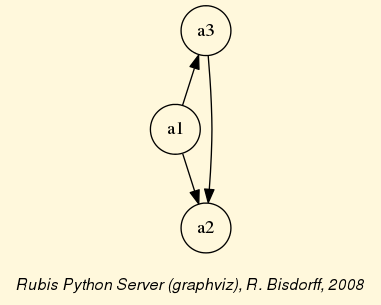
\includegraphics[width=6cm]{Figures/tutorialLinearBallots.png}
\caption{Visualizing an election result. In the Figure we notice that the \emph{majority margins} digraph from our example linear voting profile gives a linear order of the candidates: $a_1 > a_3 > a_2$, the same actually as given by the \emph{Borda} scores (see Listing \ref{list:7.4}). This is by far not given in general. Usually, when aggregating linear ballots, there appear cyclic social preferences.
}
\label{fig:7.1}       % Give a unique label
\end{figure}

\section{Cyclic social preferences}
\label{sec:7.4}

Let us consider for instance the following linear voting profile $v$ and construct the corresponding majority margins digraph.
\begin{lstlisting}[caption={Example of cyclic social preferences},label=list:7.6]
>>> v.showLinearBallots()
   voters(weight): candidates rankings
    v1(1): ['a1', 'a3', 'a5', 'a2', 'a4']
    v2(1): ['a1', 'a2', 'a4', 'a3', 'a5']
    v3(1): ['a5', 'a2', 'a4', 'a3', 'a1']
    v4(1): ['a3', 'a4', 'a1', 'a5', 'a2']
    v5(1): ['a4', 'a2', 'a3', 'a5', 'a1']
    v6(1): ['a2', 'a4', 'a5', 'a1', 'a3']
    v7(1): ['a5', 'a4', 'a3', 'a1', 'a2']
    v8(1): ['a2', 'a4', 'a5', 'a1', 'a3']
    v9(1): ['a5', 'a3', 'a4', 'a1', 'a2']
>>> mmdg = MajorityMarginsDigraph(v)
>>> mmdg.showRelationTable()
    * ---- Relation Table -----
      S   |  'v1'   'v2'   'v3'	  'v4'	  'v5'	  
    ------|----------------------------------------
    'v1'  |   -     0.11  -0.11	 -0.56	 -0.33	 
    'v2'  | -0.11    -	   0.11	  0.11	 -0.11	 
    'v3'  |  0.11  -0.11    -	 -0.33	 -0.11	 
    'v4'  |  0.56  -0.11   0.33	   -	  0.11	 
    'v5'  |  0.33   0.11   0.11	 -0.11	   -	 
\end{lstlisting}    
Now, we cannot find any completely positive row in the relation table (see Listing \ref{list:7.6} Lines 17 - ). No one of the five candidates is beating all the others with an absolute majority of votes. There is no \emph{Condorcet} winner anymore. In fact, when looking at a graphviz drawing of this \emph{majority margins} digraph, we may observe \textbf{cyclic} preferences, like $(v_1 > v_2 > v_3 > v_1)$ for instance.
\begin{lstlisting}
>>> mmdg.exportGraphViz('cycles')
 *---- exporting a dot file for GraphViz tools ---------*
  Exporting to cycles.dot
  dot -Grankdir=BT -Tpng cycles.dot -o cycles.png
\end{lstlisting}
\begin{figure}[h]
\sidecaption[t]
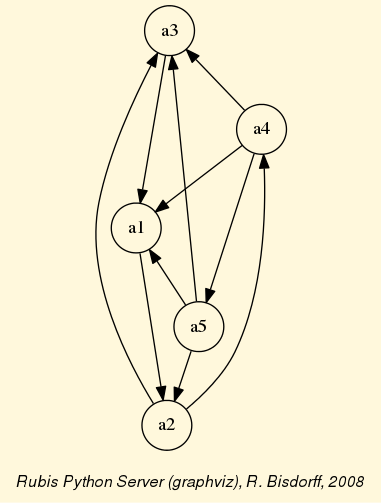
\includegraphics[width=4cm]{Figures/cycles.png}
\caption{Cyclic social preferences.}
\label{fig:7.2}       % Give a unique label
\end{figure}
	   
But, there may be many cycles appearing in a \emph{majority margins} digraph, and, we may detect and enumerate all minimal chordless circuits in a Digraph instance with the \texttt{computeChordlessCircuits} method.\index{computeChordlessCircuits}
\begin{lstlisting}
>>> mmdg.computeChordlessCircuits()
 [(['a2', 'a3', 'a1'], frozenset({'a2', 'a3', 'a1'})), 
  (['a2', 'a4', 'a5'], frozenset({'a2', 'a5', 'a4'})), 
  (['a2', 'a4', 'a1'], frozenset({'a2', 'a1', 'a4'}))]
\end{lstlisting}

\Condorcet 's approach for determining the winner of an election is hence \emph{not decisive} in all circumstances and we need to exploit more sophisticated approaches for finding the winner of the election on the basis of the majority margins of the given linear ballots (see Chapter ref{sec:8} and \citet{BIS-2008a}). 

Many more tools for exploiting voting results are available like the browser heat map view on voting profiles\index{showHTMLVotingHeatmap@\texttt{showHTMLVotingHeatmap()}}. The number of voters is usually much larger than the number of candidates. In that case, it is better to generate a transposed \emph{voters} $\times$ \emph{candidates} view (see Line 2 below) 
\begin{lstlisting}
>>> v.showHTMLVotingHeatmap(rankingRule='NetFlows',
...                         Transposed=False)
\end{lstlisting}
\begin{figure}[h]
\sidecaption[t]
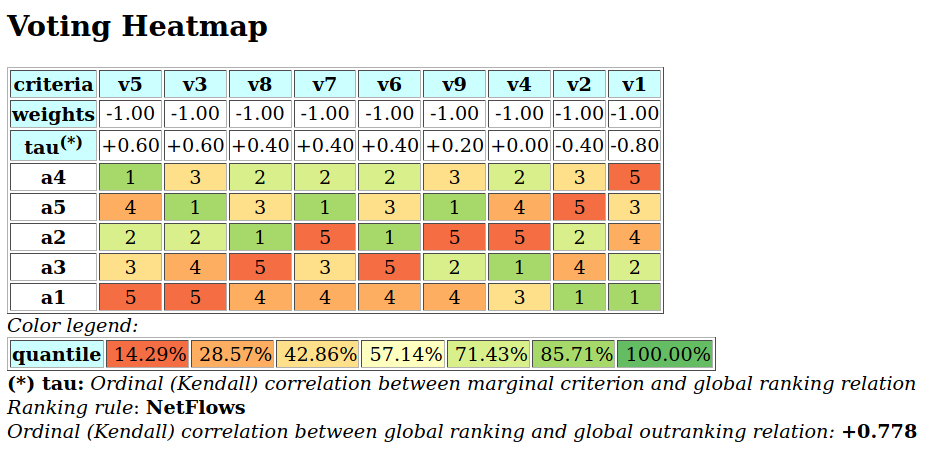
\includegraphics[width=4cm]{Figures/votingHeatmap.png}
\caption{Visualizing a linear voting profile in a heatmap format. Notice that the importance weights of the voters are \emph{negative}, which means that the preference direction of the criteria (in this case the individual voters) is \emph{decreasing}, i.e. goes from lowest (best) rank to highest (worst) rank.
}
\label{fig:7.3}       % Give a unique label
\end{figure}

It worthwhile noticing that the compromise \emph{NetFlows} ranking \texttt{a4} $>$ \texttt{a5} $>$ \texttt{a2} $>$ \texttt{a1} $>$ \texttt{a3}, shown in this heatmap (see Fig. \ref{fig:7.3}) results in an optimal \emph{ordinal correlation} index of $+0.778$ with the pairwise majority voting margins (see Chapter \ref{sec:16}). 

\section{On generating realistic random linear voting profiles}
\label{sec:7.5}

By default, the \texttt{RandomLinearVotingProfile} class generates random linear voting profiles where every candidates has the same uniform probabilities to be ranked at a certain position by all the voters. Each voter's random linear ballot is indeed generated  via a uniform shuffling of the list of candidates.

In reality, political election data appear quite different. There usually will be different favorite and marginal candidates for each political party. To simulate these aspects into our random generator, we are using two random exponentially distributed polls of the candidates and consider a bipartisan political landscape with a certain random balance (default theoretical party repartition = $0.50$) between the two sets of potential party supporters. A certain theoretical proportion (default = $0.1$) will not support any party.

Let us generate such a linear voting profile for an election with $1000$ voters and $15$ candidates.

\begin{lstlisting}[caption={Generating a linear voting profile with random polls},label=list:7.7]
>>> from votingProfiles import\
...            RandomLinearVotingProfile
>>> lvp = RandomLinearVotingProfile(\
...         numberOfCandidates=15,
...         numberOfVoters=1000,
...         WithPolls=True,
...         partyRepartition=0.5,
...         other=0.1,
...         seed=0.9189670954954139)
>>> lvp
 *------- VotingProfile instance description ------*
  Instance class : RandomLinearVotingProfile
  Instance name  : randLinearProfile
  Candidates     : 15
  Voters         : 1000
  Attributes     : ['name', 'seed', 'candidates',
                    'voters', 'RandomWeights',
                    'sumWeights', 'poll1', 'poll2',
                    'bipartisan', 'linearBallot',
                    'ballot']
>>> lvp.showRandomPolls()
  Random repartition of voters
   Party_1 supporters : 460 (46.0%)
   Party_2 supporters : 436 (43.6%)
   Other voters       : 104 (10.4%)
 *---------------- random polls ----------------*
   Party-1(46.0%) | Party-2(43.6%)|  expected  
  ----------------------------------------------
    a06 : 19.91%  | a11 : 22.94%  | a06 : 15.00%
    a07 : 14.27%  | a08 : 15.65%  | a11 : 13.08%
    a03 : 10.02%  | a04 : 15.07%  | a08 : 09.01%
    a13 : 08.39%  | a06 : 13.40%  | a07 : 08.79%
    a15 : 08.39%  | a03 : 06.49%  | a03 : 07.44%
    a11 : 06.70%  | a09 : 05.63%  | a04 : 07.11%
    a01 : 06.17%  | a07 : 05.10%  | a01 : 05.06%
    a12 : 04.81%  | a01 : 05.09%  | a13 : 05.04%
    a08 : 04.75%  | a12 : 03.43%  | a15 : 04.23%
    a10 : 04.66%  | a13 : 02.71%  | a12 : 03.71%
    a14 : 04.42%  | a14 : 02.70%  | a14 : 03.21%
    a05 : 04.01%  | a15 : 00.86%  | a09 : 03.10%
    a09 : 01.40%  | a10 : 00.44%  | a10 : 02.34%
    a04 : 01.18%  | a05 : 00.29%  | a05 : 01.97%
    a02 : 00.90%  | a02 : 00.21%  | a02 : 00.51%
\end{lstlisting}

In this example (see Listing \ref{list:7.7} Lines 18-), we obtain 460 Party-1 supporters ($46\%$), 436 Party-2 supporters ($43.6\%$) and 104 other voters ($10.4\%$). Favorite candidates of Party-1 supporters, with more than $10\%$, appear to be \texttt{a06} ($19.91\%$), $a07$ ($14.27\%$) and \texttt{a03} ($10.02\%$). Whereas for Party-2 supporters, favorite candidates appear to be \texttt{a11} ($22.94\%$), followed by \texttt{a08} ($15.65\%$), $a04$ ($15.07\%$) and \texttt{a06} ($13.4\%$). Being \emph{first} choice for Party-1 supporters and \emph{fourth} choice for Party-2 supporters, this candidate \texttt{a06} is a natural candidate for clearly winning this election game (see Listing \ref{list:7.8}).
\begin{lstlisting}[caption={The uninominal and \emph{Borda} election winner},label=list:7.8]
>>> lvp.computeSimpleMajorityWinner()
 ['a06']
>>> lvp.computeInstantRunoffWinner()
 ['a06']  
>>> lvp.computeBordaWinners()
 ['a06']
\end{lstlisting}

Is it also a \Condorcet winner ? To verify, we start by creating the corresponding \emph{majority margins} digraph $mmdg$ with the help of the \texttt{MajorityMarginsDigraph} class. The created digraph instance contains 15 \emph{actions} --the candidates-- and 105 \emph{oriented arcs} --the \emph{positive} majority margins-- (see Listing \ref{list:7.9} Lines 7-8).
\begin{lstlisting}[caption={A majority margins digraph constructed from a linear voting profile},label=list:7.9]
>>> from votingProfiles import MajorityMarginsDigraph
>>> mmdg = MajorityMarginsDigraph(lvp)
>>> mmdg
 *------- Digraph instance description ------*
  Instance class      : MajorityMarginsDigraph
  Instance name       : rel_randLinearProfile
  Digraph Order       : 15
  Digraph Size        : 104
  Valuation domain    : [-1000.00;1000.00]
  Determinateness (%) : 67.08
  Attributes          : ['name', 'actions', 'voters',
                         'ballot', 'valuationdomain',
                         'relation', 'order',
                         'gamma', 'notGamma']
\end{lstlisting}

We may visualize the resulting pairwise majority margins by showing the HTML formated version of the $mmdg$ relation table in a browser view.
\begin{lstlisting}
>>> cdg.showHTMLRelationTable(\
...         tableTitle='Pairwise majority margins',
...         relationName='M(x>y)')
\end{lstlisting}
\begin{figure}[h]
\sidecaption[t]
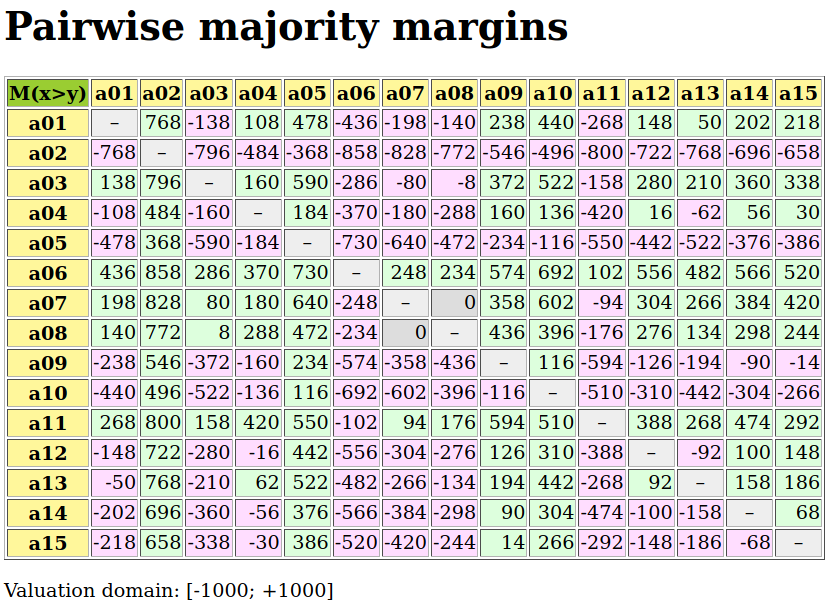
\includegraphics[width=4cm]{Figures/majorityMargins.png}
\caption{Browsing the majority margins. \emph{Light green} cells contain the positive majority margins, whereas \emph{light red} cells contain the negative majority margins.}
\label{fig:7.4}       % Give a unique label
\end{figure}

A complete \emph{light green} row reveals a \Condorcet winner, whereas a complete \emph{light green} column reveals a \Condorcet loser. We recover again candidate \texttt{a06} as \emph{Condorcet} winner\footnote{The concept of \Condorcet winner --a generalization of absolute majority winners-- proposed by \Condorcet in 1785, is an early historical example of initial digraph kernel (see Chapter \ref{sec:17})}.), whereas the obvious \emph{Condorcet} loser is here candidate \texttt{a02}, the candidate with the lowest support in both parties (see Listing \ref{list:7.7} Line 40).

With a same \emph{bipolar-first ranked} and \emph{last ranked} candidate- selection procedure\index{computeRankingByChoosing@\texttt{computeRankingByChoosing()}}, we may \emph{weakly rank} the candidates (with possible ties) by iterating these \emph{first ranked} and \emph{last ranked} choices among the remaining candidates \citep{BIS-1999}.

Before showing the \emph{ranking-by-choosing} result, we have to compute the iterated bipolar selection procedure (see Listing \ref{list:7.10} Line 2).
\begin{lstlisting}[caption={Ranking by iterating choosing the \emph{first} and \emph{last} remaining candidates },label=list:7.10]
>>> cdg.showRankingByChoosing()
 Error: You must first run
  self.computeRankingByChoosing(CoDual=False(default)|True) !
>>> cdg.computeRankingByChoosing()
>>> cdg.showRankingByChoosing()
 Ranking by Choosing and Rejecting
   1st first ranked ['a06']
     2nd first ranked ['a11']
       3rd first ranked ['a07', 'a08']
         4th first ranked ['a03']
           5th first ranked ['a01']
             6th first ranked ['a13']
               7th first ranked ['a04']
               7th last ranked ['a12']
	     6th last ranked ['a14']
	   5th last ranked ['a15']
	 4th last ranked ['a09']
       3rd last ranked ['a10']
     2nd last ranked ['a05']
   1st last ranked ['a02']
\end{lstlisting}
The first selection concerns \texttt{a06} (first) and \texttt{a02} (last), followed by \texttt{a11} (first) opposed to \texttt{a05} (last), and so on, until there remains at iteration step 7 a last pair of candidates, namely [\texttt{a04}, \texttt{a12}] (see Lines 13-14).

Notice furthermore the first ranked candidates at iteration step 3 (see Line 9), namely the pair (\texttt{a07}, \texttt{a08}). Both candidates represent indeed conjointly the \emph{first ranked} choice. We obtain here hence a \emph{weak ranking}, i.e. a ranking with a tie.

Let us mention that the \emph{instant-run-off} procedure, we used before (see Listing \ref{list:7.8} Line 3), when operated with a \texttt{Comments=True} parameter setting, will deliver a more or less similar \emph{reversed} linear \emph{ordering-by-rejecting} result, namely \texttt{[a02, a10, a14, a05, a09, a13, a12, a15, a04, a01, a08, a03, a07, a11, a06]}, ordered from the \emph{last} to the \emph{first} choice.

Remarkable about both these \emph{ranking-by-choosing} or \emph{ordering-by-rejecting} results is the fact that the random voting behaviour, simulated here with the help of two discrete random variables \footnote{Discrete random variables with a given empirical probability law (here the polls) are provided in the \texttt{randomNumbers} module by the \texttt{DiscreteRandomVariable} class.}, defined respectively by the two party polls, is rendering a ranking that is more or less in accordance with the simulated balance of the polls: Party-1 supporters : 460;  Party-2 supporters: 436 (see Listing \ref{list:7.7} Lines 26-40 third column). Despite a random voting behaviour per voter, the given polls apparently show a \emph{very strong incidence} on the eventual election result. In order to avoid any manipulation of the election outcome, public media are therefore in some countries not allowed to publish polls during the last weeks before a general election.

Mind that the specific \emph{ranking-by-choosing} procedure, we use here on the \emph{majority margins} digraph, operates the selection procedure by extracting at each step \emph{initial} and \emph{terminal} kernels, i.e. NP-hard operational problems (see Chapter \ref{sec:17} and \citet{BIS-1999}); A technique that does not allow in general to tackle voting profiles with) much more than 30 candidates. The chapter on ranking methods (Chapter \ref{sec:8}) provides more adequate and efficient techniques for ranking from pairwise majority margins when a larger number of potential candidates is given.  

%%%%%%% The chapter bibliography
%\normallatexbib
\clearpage
%\phantomsection
%\addcontentsline{toc}{section}{Chapter Bibliography}
\bibliographystyle{spbasic}
%\typeout{}
\bibliography{03-backMatters/reference}
%\chapter{Computing the winner of an election}
\label{sec:7}

\abstract*{To be written.}
  
\abstract{To be written.}

\section{Linear voting profiles}
\label{sec:7.1}

The {\tt votingProfiles}\index{votingProfiles@\texttt{votingProfiles} module} module provides resources for handling election results \citep{ADT-L2}, like the \texttt{LinearVotingProfile} class\index{LinearVotingProfile@\texttt{LinearVotingProfile} class}. We consider an election involving a finite set of candidates and finite set of weighted voters, who express their voting preferences in a complete linear ranking (without ties) of the candidates. The data is internally stored in two ordered dictionaries, one for the voters and another one for the candidates. The linear ballots are stored in a standard dictionary.
\begin{lstlisting}
candidates = OrderedDict([
  ('a1',...), ('a2',...), ('a3', ...), ...}
voters = OrderedDict([
  ('v1',{'weight':10}),
  ('v2',{'weight':3}),
  ... ])
  # each voter specifies a
  # linearly ranked list of candidates
  # from the best to the worst (without ties
linearBallot = {
  'v1' : ['a2','a3','a1', ...],
  'v2' : ['a1','a2','a3', ...],
   ...
  }
\end{lstlisting}

The module provides a \texttt{RandomLinearVotingProfile} class \index{RandomLinearVotingProfile@\texttt{RandomLinearVotingProfile} class} for generating random instances of the \texttt{LinearVotingProfile} class. In an interactive Python session we may obtain for the election of 3 candidates by 5 voters the following result.
\begin{lstlisting}[caption={Example of random linear voting profile},label=list:7.1]
>>> from votingProfiles import\
...              RandomLinearVotingProfile
>>> lvp = RandomLinearVotingProfile(numberOfVoters=5,\
...                               numberOfCandidates=3,\
...                               RandomWeights=True) 
>>> lvp.candidates
  OrderedDict([ ('a1',{'name':'a1}),
                ('a2',{'name':'a2'}),
                ('a3',{'name':'a3'}) ])
>>> lvp.voters
  OrderedDict([('v1',{'weight': 2}),
               ('v2':{'weight': 3}), 
               ('v3',{'weight': 1}),
               ('v4':{'weight': 5}),
               ('v5',{'weight': 4})])
>>> lvp.linearBallot
    {'v1': ['a1', 'a2', 'a3',],
     'v2': ['a3', 'a2', 'a1',],
     'v3': ['a1', 'a3', 'a2',],
     'v4': ['a1', 'a3', 'a2',],
     'v5': ['a2', 'a3', 'a1',]} 
 \end{lstlisting}

Notice that in this random example, the five voters are weighted (see Listing \ref{list:7.1} Line 6-7). Their linear ballots can be viewed with the \texttt{showLinearBallots}\index{()showLinearBallots@\texttt{showLinearBallots}} method.
\begin{lstlisting}
>>> lvp.showLinearBallots()
    voters(weight)	 candidates rankings
    v1(2): 	 ['a2', 'a1', 'a3']
    v2(3): 	 ['a3', 'a1', 'a2']
    v3(1): 	 ['a1', 'a3', 'a2']
    v4(5): 	 ['a1', 'a2', 'a3']
    v5(4): 	 ['a3', 'a1', 'a2']
    nbr. of voters: 15
\end{lstlisting}

Editing of the linear voting profile may be achieved by storing the data in a file, edit it, and reload it again.
\begin{lstlisting}
>>> v.save(fileName='tutorialLinearVotingProfile1')
   *--- Saving linear profile in file:
                   <tutorialLinearVotingProfile1.py> ---*
>>> from votingProfiles import LinearVotingProfile
>>> v = LinearVotingProfile('tutorialLinearVotingProfile1')
\end{lstlisting}

\section{Computing the winner}
\label{sec:7.2}

We may easily compute \emph{uninominal votes}\index{uninominal votes}, i.e. how many times a candidate was ranked first, and see who is consequently the \emph{simple majority} (plurality) winner(s) in this election.
\begin{lstlisting}
>>> v.computeUninominalVotes()
  {'a2': 2, 'a1': 6, 'a3': 7}
>>> v.computeSimpleMajorityWinner()
  ['a3']
\end{lstlisting}

As we observe no absolute majority (8/15) of votes for any of the three candidate, we may look for the \emph{instant runoff} winner\index{computeInstantRunoffWinner@\texttt{computeInstantRunoffWinner()}} instead (see \citet{ADT-L2}).
\begin{lstlisting}[caption={Example Instant Run Off Winner},label=list:7.2]
>>> v.computeInstantRunoffWinner(Comments=True)
  Half of the Votes =  7.50
    ==> stage =  1
	remaining candidates ['a1', 'a2', 'a3']
	uninominal votes {'a1': 6, 'a2': 2, 'a3': 7}
	minimal number of votes =  2
	maximal number of votes =  7
	candidate to remove =  a2
	remaining candidates =  ['a1', 'a3']
    ==> stage =  2
	remaining candidates ['a1', 'a3']
	uninominal votes {'a1': 8, 'a3': 7}
	minimal number of votes =  7
	maximal number of votes =  8
	candidate a1 obtains an absolute majority
   Instant run off winner: ['a1']
 \end{lstlisting}
In stage 1, no candidate obtains an absolute majority of votes. Candidate \texttt{a2} obtains the minimal number of votes (2/15) and is, hence, eliminated. In stage 2, candidate \texttt{a1} obtains an absolute majority of the votes (8/15) and is eventually elected (see Listing \ref{list:7.2}).

We may also follow the \emph{Chevalier de Borda}'s advice and, after a \textbf{rank analysis} of the linear ballots, compute the \emph{Borda score} -the average rank- of each candidate and hence determine the \emph{Borda winner(s)}\index{computeRankAnalysis@\texttt{computeRankAnalysis()}}.
\begin{lstlisting}[caption={Example of \emph{Borda} rank scores},label=list:7.3]
>>> v.computeRankAnalysis()
 {'a2': [2, 5, 8], 'a1': [6, 9, 0], 'a3': [7, 1, 7]}
>>> v.computeBordaScores()
 OrderedDict([
   ('a1', {'BordaScore': 24, 'averageBordaScore': 1.6}),
   ('a3', {'BordaScore': 30, 'averageBordaScore': 2.0}),
   ('a2', {'BordaScore': 36, 'averageBordaScore': 2.4}) ])
>>> v.computeBordaWinners()
 ['a1']
\end{lstlisting}
Candidate \texttt{a1} obtains the minimal \emph{Borda} score, followed by candidate \texttt{a3} and finally candidate \texttt{a2} (see Listing \ref{list:7.3}). The corresponding \emph{Borda rank analysis table} may be printed out with a corresponding \texttt{showRankAnalysisTable()} command \index{showRankAnalysisTable@\texttt{showRankAnalysisTable()}}.
\begin{lstlisting}[caption={Rank analysis example},label=list:7.4]
>>> v.showRankAnalysisTable()
 *----  Borda rank analysis tableau -----*
  candi- | alternative-to-rank |     Borda
  dates  |   1     2     3     | score  average
  -------|-------------------------------------
   'a1'  |   6     9     0     | 24/15   1.60
   'a3'  |   7     1     7     | 30/15   2.00
   'a2'  |   2     5     8     | 36/15   2.40
 \end{lstlisting}

In our randomly generated election results, we are lucky: The instant runoff winner and the \emph{Borda} winner both is candidate \texttt{a1} (see Listings \ref{list:7.2} and \ref{list:7.3}). However, we could also follow the \emph{Marquis de Condorcet}'s advice, and compute the \emph{majority margins} obtained by voting for each individual pair of candidates.

\section{The majority margins digraph}
\label{sec:7.3}

For instance, candidate \texttt{a1} is ranked four times before and once behind candidate \texttt{a2}. Hence the corresponding \emph{majority margin}\index{majority margins} $M(a_1,a_2)$ is $4 - 1 = +3$. These \emph{majority margins} define on the set of candidates what we call the \emph{majority margins digraph}\index{majority margins digraph}. The \texttt{MajorityMarginsDigraph} class\index{MajorityMarginsDigraph@\texttt{MajorityMarginsDigraph} class} (a specialization of the root \texttt{Digraph} class) is available for handling such kind of digraphs.
\begin{lstlisting}[caption={Example of \emph{Majority Margins} digraph},label=list:7.5]
>>> from votingProfiles import MajorityMarginsDigraph
>>> mmdg = MajorityMarginsDigraph(lvp,\
...                IntegerValuation=True)
>>> mmdg
 *------- Digraph instance description ------*
  Instance class      : MajorityMarginsDigraph
  Instance name       : rel_randomLinearVotingProfile1
  Digraph Order       : 3
  Digraph Size        : 3
  Valuation domain    : [-15.00;15.00]
  Determinateness (%) : 64.44
  Attributes          : ['name', 'actions', 'voters',
                         'ballot', 'valuationdomain',
                         'relation', 'order',
                         'gamma', 'notGamma']
>>> mmdg.showAll()
 *----- show detail -------------*
  Digraph          : rel_randLinearVotingProfile1
  *---- Actions ----*
   ['a1', 'a2', 'a3']
  *---- Characteristic valuation domain ----*
  {'max': Decimal('15.0'),
   'med': Decimal('0'),
   'min': Decimal('-15.0'),
   'hasIntegerValuation': True}
  *---- majority margins -----*
     M(x,y) |  'a1'   'a2'  'a3'	  
    --------|-------------------
      'a1'  |    0     11     1	 
      'a2'  |  -11      0    -1	 
      'a3'  |   -1      1     0	 
    Valuation domain: [-15;+15]
\end{lstlisting}

Notice that, in the case of linear voting profiles, majority margins always verify a \emph{zero sum property}: $M(x,y) + M(y,x) = 0$ for all candidates $x$ and $y$ (see Listing \ref{list:7.5} Lines 26-28). This is not true in general for arbitrary voting profiles. The \emph{majority margins} digraph of linear voting profiles defines in fact a \emph{weak tournament}\index{weak tournament} and belongs, hence, to the class of \emph{self-codual} bipolar-valued digraphs\footnote{The class of self-codual bipolar-valued digraphs consists of all weakly asymmetric digraphs, i.e. digraphs containing only asymmetric and/or indeterminate links. Limit cases consists of, on the one side, full tournaments with indeterminate reflexive links, and, on the other side, fully indeterminate digraphs. In this class, the converse (inverse $\sim$) operator is indeed identical to the dual (negation $-$ ) one.}.
    
Now, a candidate $x$, showing a positive majority margin $M(x,y)$, is beating candidate $y$  with an absolute majority in a pairwise voting. Hence, a candidate showing only positive terms in her row in the \emph{majority margins} digraph relation table, beats all other candidates with absolute majority of votes. \Condorcet recommends to declare this candidate (is always unique, why?) the winner of the election. Here we are lucky, it is again candidate \texttt{a1} who is hence the \emph{Condorcet winner}\index{Condorcet!winner} (see Listing \ref{list:7.5} Line 26).
\begin{lstlisting}
>>> mmdg.computeCondorcetWinners()
 ['a1']  
\end{lstlisting}    

By seeing the majority margins like a \emph{bipolar-valued characteristic function} of a global preference relation defined on the set of candidates, we may use all operational resources of the generic \texttt{Digraph} class (see Chapter \ref{sec:2}), and especially its \texttt{exportGraphViz()} method \footnote{The \texttt{exportGraphViz()} method is depending on drawing tools from the graphviz software (https://graphviz.org/).}, for visualizing an election result.
\begin{lstlisting}
>>> mmdg.exportGraphViz(fileName='tutorialLinearBallots')
 *---- exporting a dot file for GraphViz tools ---------*
  Exporting to tutorialLinearBallots.dot
  dot -Grankdir=BT -Tpng tutorialLinearBallots.dot \
                   -o tutorialLinearBallots.png
\end{lstlisting}
\begin{figure}[h]
\sidecaption[t]
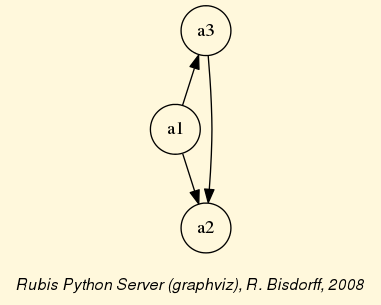
\includegraphics[width=6cm]{Figures/tutorialLinearBallots.png}
\caption{Visualizing an election result. In the Figure we notice that the \emph{majority margins} digraph from our example linear voting profile gives a linear order of the candidates: $a_1 > a_3 > a_2$, the same actually as given by the \emph{Borda} scores (see Listing \ref{list:7.4}). This is by far not given in general. Usually, when aggregating linear ballots, there appear cyclic social preferences.
}
\label{fig:7.1}       % Give a unique label
\end{figure}

\section{Cyclic social preferences}
\label{sec:7.4}

Let us consider for instance the following linear voting profile $v$ and construct the corresponding majority margins digraph.
\begin{lstlisting}[caption={Example of cyclic social preferences},label=list:7.6]
>>> v.showLinearBallots()
   voters(weight): candidates rankings
    v1(1): ['a1', 'a3', 'a5', 'a2', 'a4']
    v2(1): ['a1', 'a2', 'a4', 'a3', 'a5']
    v3(1): ['a5', 'a2', 'a4', 'a3', 'a1']
    v4(1): ['a3', 'a4', 'a1', 'a5', 'a2']
    v5(1): ['a4', 'a2', 'a3', 'a5', 'a1']
    v6(1): ['a2', 'a4', 'a5', 'a1', 'a3']
    v7(1): ['a5', 'a4', 'a3', 'a1', 'a2']
    v8(1): ['a2', 'a4', 'a5', 'a1', 'a3']
    v9(1): ['a5', 'a3', 'a4', 'a1', 'a2']
>>> mmdg = MajorityMarginsDigraph(v)
>>> mmdg.showRelationTable()
    * ---- Relation Table -----
      S   |  'v1'   'v2'   'v3'	  'v4'	  'v5'	  
    ------|----------------------------------------
    'v1'  |   -     0.11  -0.11	 -0.56	 -0.33	 
    'v2'  | -0.11    -	   0.11	  0.11	 -0.11	 
    'v3'  |  0.11  -0.11    -	 -0.33	 -0.11	 
    'v4'  |  0.56  -0.11   0.33	   -	  0.11	 
    'v5'  |  0.33   0.11   0.11	 -0.11	   -	 
\end{lstlisting}    
Now, we cannot find any completely positive row in the relation table (see Listing \ref{list:7.6} Lines 17 - ). No one of the five candidates is beating all the others with an absolute majority of votes. There is no \emph{Condorcet} winner anymore. In fact, when looking at a graphviz drawing of this \emph{majority margins} digraph, we may observe \textbf{cyclic} preferences, like $(v_1 > v_2 > v_3 > v_1)$ for instance.
\begin{lstlisting}
>>> mmdg.exportGraphViz('cycles')
 *---- exporting a dot file for GraphViz tools ---------*
  Exporting to cycles.dot
  dot -Grankdir=BT -Tpng cycles.dot -o cycles.png
\end{lstlisting}
\begin{figure}[h]
\sidecaption[t]
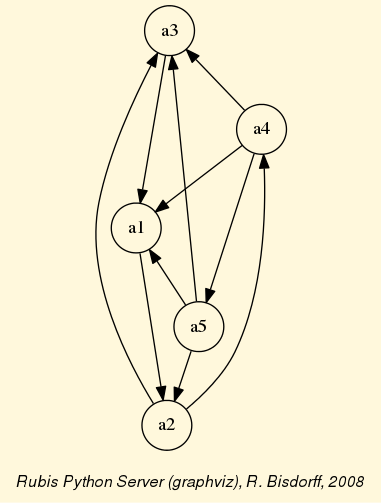
\includegraphics[width=4cm]{Figures/cycles.png}
\caption{Cyclic social preferences.}
\label{fig:7.2}       % Give a unique label
\end{figure}
	   
But, there may be many cycles appearing in a \emph{majority margins} digraph, and, we may detect and enumerate all minimal chordless circuits in a Digraph instance with the \texttt{computeChordlessCircuits} method.\index{computeChordlessCircuits}
\begin{lstlisting}
>>> mmdg.computeChordlessCircuits()
 [(['a2', 'a3', 'a1'], frozenset({'a2', 'a3', 'a1'})), 
  (['a2', 'a4', 'a5'], frozenset({'a2', 'a5', 'a4'})), 
  (['a2', 'a4', 'a1'], frozenset({'a2', 'a1', 'a4'}))]
\end{lstlisting}

\Condorcet 's approach for determining the winner of an election is hence \emph{not decisive} in all circumstances and we need to exploit more sophisticated approaches for finding the winner of the election on the basis of the majority margins of the given linear ballots (see Chapter ref{sec:8} and \citet{BIS-2008a}). 

Many more tools for exploiting voting results are available like the browser heat map view on voting profiles\index{showHTMLVotingHeatmap@\texttt{showHTMLVotingHeatmap()}}. The number of voters is usually much larger than the number of candidates. In that case, it is better to generate a transposed \emph{voters} $\times$ \emph{candidates} view (see Line 2 below) 
\begin{lstlisting}
>>> v.showHTMLVotingHeatmap(rankingRule='NetFlows',
...                         Transposed=False)
\end{lstlisting}
\begin{figure}[h]
\sidecaption[t]
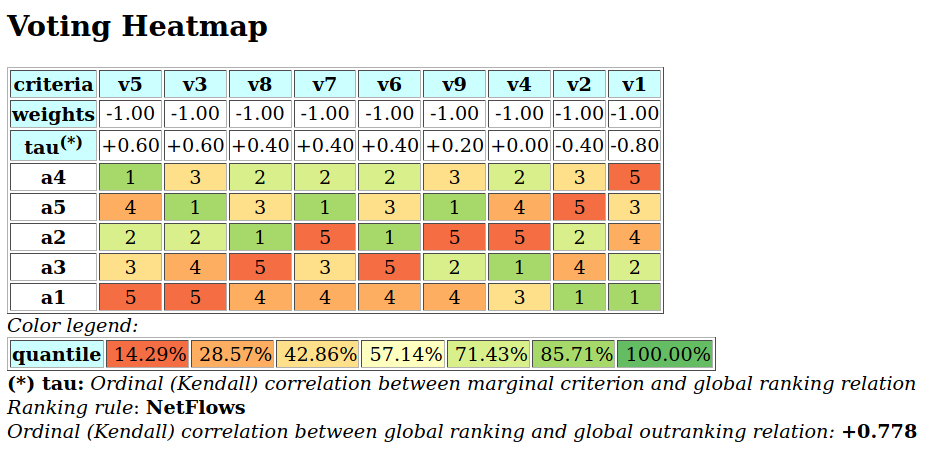
\includegraphics[width=4cm]{Figures/votingHeatmap.png}
\caption{Visualizing a linear voting profile in a heatmap format. Notice that the importance weights of the voters are \emph{negative}, which means that the preference direction of the criteria (in this case the individual voters) is \emph{decreasing}, i.e. goes from lowest (best) rank to highest (worst) rank.
}
\label{fig:7.3}       % Give a unique label
\end{figure}

It worthwhile noticing that the compromise \emph{NetFlows} ranking \texttt{a4} $>$ \texttt{a5} $>$ \texttt{a2} $>$ \texttt{a1} $>$ \texttt{a3}, shown in this heatmap (see Fig. \ref{fig:7.3}) results in an optimal \emph{ordinal correlation} index of $+0.778$ with the pairwise majority voting margins (see Chapter \ref{sec:16}). 

\section{On generating realistic random linear voting profiles}
\label{sec:7.5}

By default, the \texttt{RandomLinearVotingProfile} class generates random linear voting profiles where every candidates has the same uniform probabilities to be ranked at a certain position by all the voters. Each voter's random linear ballot is indeed generated  via a uniform shuffling of the list of candidates.

In reality, political election data appear quite different. There usually will be different favorite and marginal candidates for each political party. To simulate these aspects into our random generator, we are using two random exponentially distributed polls of the candidates and consider a bipartisan political landscape with a certain random balance (default theoretical party repartition = $0.50$) between the two sets of potential party supporters. A certain theoretical proportion (default = $0.1$) will not support any party.

Let us generate such a linear voting profile for an election with $1000$ voters and $15$ candidates.

\begin{lstlisting}[caption={Generating a linear voting profile with random polls},label=list:7.7]
>>> from votingProfiles import\
...            RandomLinearVotingProfile
>>> lvp = RandomLinearVotingProfile(\
...         numberOfCandidates=15,
...         numberOfVoters=1000,
...         WithPolls=True,
...         partyRepartition=0.5,
...         other=0.1,
...         seed=0.9189670954954139)
>>> lvp
 *------- VotingProfile instance description ------*
  Instance class : RandomLinearVotingProfile
  Instance name  : randLinearProfile
  Candidates     : 15
  Voters         : 1000
  Attributes     : ['name', 'seed', 'candidates',
                    'voters', 'RandomWeights',
                    'sumWeights', 'poll1', 'poll2',
                    'bipartisan', 'linearBallot',
                    'ballot']
>>> lvp.showRandomPolls()
  Random repartition of voters
   Party_1 supporters : 460 (46.0%)
   Party_2 supporters : 436 (43.6%)
   Other voters       : 104 (10.4%)
 *---------------- random polls ----------------*
   Party-1(46.0%) | Party-2(43.6%)|  expected  
  ----------------------------------------------
    a06 : 19.91%  | a11 : 22.94%  | a06 : 15.00%
    a07 : 14.27%  | a08 : 15.65%  | a11 : 13.08%
    a03 : 10.02%  | a04 : 15.07%  | a08 : 09.01%
    a13 : 08.39%  | a06 : 13.40%  | a07 : 08.79%
    a15 : 08.39%  | a03 : 06.49%  | a03 : 07.44%
    a11 : 06.70%  | a09 : 05.63%  | a04 : 07.11%
    a01 : 06.17%  | a07 : 05.10%  | a01 : 05.06%
    a12 : 04.81%  | a01 : 05.09%  | a13 : 05.04%
    a08 : 04.75%  | a12 : 03.43%  | a15 : 04.23%
    a10 : 04.66%  | a13 : 02.71%  | a12 : 03.71%
    a14 : 04.42%  | a14 : 02.70%  | a14 : 03.21%
    a05 : 04.01%  | a15 : 00.86%  | a09 : 03.10%
    a09 : 01.40%  | a10 : 00.44%  | a10 : 02.34%
    a04 : 01.18%  | a05 : 00.29%  | a05 : 01.97%
    a02 : 00.90%  | a02 : 00.21%  | a02 : 00.51%
\end{lstlisting}

In this example (see Listing \ref{list:7.7} Lines 18-), we obtain 460 Party-1 supporters ($46\%$), 436 Party-2 supporters ($43.6\%$) and 104 other voters ($10.4\%$). Favorite candidates of Party-1 supporters, with more than $10\%$, appear to be \texttt{a06} ($19.91\%$), $a07$ ($14.27\%$) and \texttt{a03} ($10.02\%$). Whereas for Party-2 supporters, favorite candidates appear to be \texttt{a11} ($22.94\%$), followed by \texttt{a08} ($15.65\%$), $a04$ ($15.07\%$) and \texttt{a06} ($13.4\%$). Being \emph{first} choice for Party-1 supporters and \emph{fourth} choice for Party-2 supporters, this candidate \texttt{a06} is a natural candidate for clearly winning this election game (see Listing \ref{list:7.8}).
\begin{lstlisting}[caption={The uninominal and \emph{Borda} election winner},label=list:7.8]
>>> lvp.computeSimpleMajorityWinner()
 ['a06']
>>> lvp.computeInstantRunoffWinner()
 ['a06']  
>>> lvp.computeBordaWinners()
 ['a06']
\end{lstlisting}

Is it also a \Condorcet winner ? To verify, we start by creating the corresponding \emph{majority margins} digraph $mmdg$ with the help of the \texttt{MajorityMarginsDigraph} class. The created digraph instance contains 15 \emph{actions} --the candidates-- and 105 \emph{oriented arcs} --the \emph{positive} majority margins-- (see Listing \ref{list:7.9} Lines 7-8).
\begin{lstlisting}[caption={A majority margins digraph constructed from a linear voting profile},label=list:7.9]
>>> from votingProfiles import MajorityMarginsDigraph
>>> mmdg = MajorityMarginsDigraph(lvp)
>>> mmdg
 *------- Digraph instance description ------*
  Instance class      : MajorityMarginsDigraph
  Instance name       : rel_randLinearProfile
  Digraph Order       : 15
  Digraph Size        : 104
  Valuation domain    : [-1000.00;1000.00]
  Determinateness (%) : 67.08
  Attributes          : ['name', 'actions', 'voters',
                         'ballot', 'valuationdomain',
                         'relation', 'order',
                         'gamma', 'notGamma']
\end{lstlisting}

We may visualize the resulting pairwise majority margins by showing the HTML formated version of the $mmdg$ relation table in a browser view.
\begin{lstlisting}
>>> cdg.showHTMLRelationTable(\
...         tableTitle='Pairwise majority margins',
...         relationName='M(x>y)')
\end{lstlisting}
\begin{figure}[h]
\sidecaption[t]
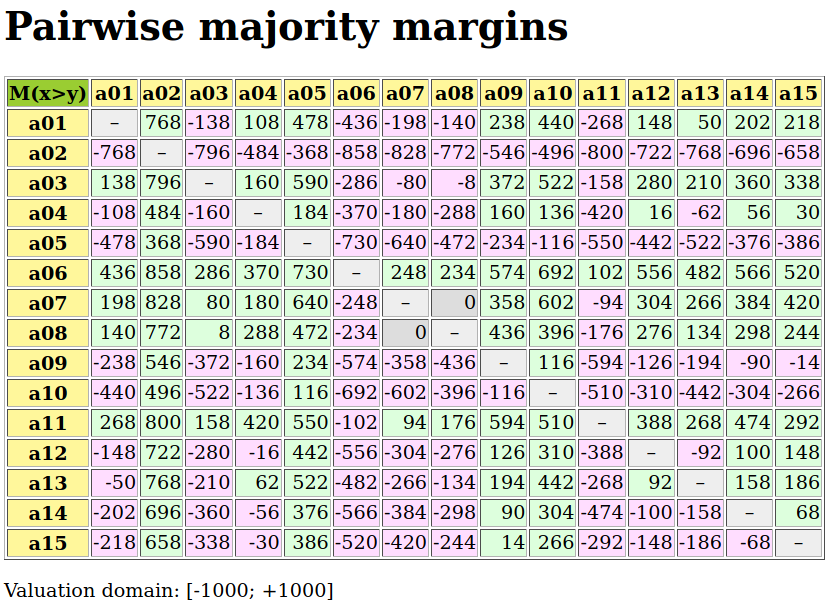
\includegraphics[width=4cm]{Figures/majorityMargins.png}
\caption{Browsing the majority margins. \emph{Light green} cells contain the positive majority margins, whereas \emph{light red} cells contain the negative majority margins.}
\label{fig:7.4}       % Give a unique label
\end{figure}

A complete \emph{light green} row reveals a \Condorcet winner, whereas a complete \emph{light green} column reveals a \Condorcet loser. We recover again candidate \texttt{a06} as \emph{Condorcet} winner\footnote{The concept of \Condorcet winner --a generalization of absolute majority winners-- proposed by \Condorcet in 1785, is an early historical example of initial digraph kernel (see Chapter \ref{sec:17})}.), whereas the obvious \emph{Condorcet} loser is here candidate \texttt{a02}, the candidate with the lowest support in both parties (see Listing \ref{list:7.7} Line 40).

With a same \emph{bipolar-first ranked} and \emph{last ranked} candidate- selection procedure\index{computeRankingByChoosing@\texttt{computeRankingByChoosing()}}, we may \emph{weakly rank} the candidates (with possible ties) by iterating these \emph{first ranked} and \emph{last ranked} choices among the remaining candidates \citep{BIS-1999}.

Before showing the \emph{ranking-by-choosing} result, we have to compute the iterated bipolar selection procedure (see Listing \ref{list:7.10} Line 2).
\begin{lstlisting}[caption={Ranking by iterating choosing the \emph{first} and \emph{last} remaining candidates },label=list:7.10]
>>> cdg.showRankingByChoosing()
 Error: You must first run
  self.computeRankingByChoosing(CoDual=False(default)|True) !
>>> cdg.computeRankingByChoosing()
>>> cdg.showRankingByChoosing()
 Ranking by Choosing and Rejecting
   1st first ranked ['a06']
     2nd first ranked ['a11']
       3rd first ranked ['a07', 'a08']
         4th first ranked ['a03']
           5th first ranked ['a01']
             6th first ranked ['a13']
               7th first ranked ['a04']
               7th last ranked ['a12']
	     6th last ranked ['a14']
	   5th last ranked ['a15']
	 4th last ranked ['a09']
       3rd last ranked ['a10']
     2nd last ranked ['a05']
   1st last ranked ['a02']
\end{lstlisting}
The first selection concerns \texttt{a06} (first) and \texttt{a02} (last), followed by \texttt{a11} (first) opposed to \texttt{a05} (last), and so on, until there remains at iteration step 7 a last pair of candidates, namely [\texttt{a04}, \texttt{a12}] (see Lines 13-14).

Notice furthermore the first ranked candidates at iteration step 3 (see Line 9), namely the pair (\texttt{a07}, \texttt{a08}). Both candidates represent indeed conjointly the \emph{first ranked} choice. We obtain here hence a \emph{weak ranking}, i.e. a ranking with a tie.

Let us mention that the \emph{instant-run-off} procedure, we used before (see Listing \ref{list:7.8} Line 3), when operated with a \texttt{Comments=True} parameter setting, will deliver a more or less similar \emph{reversed} linear \emph{ordering-by-rejecting} result, namely \texttt{[a02, a10, a14, a05, a09, a13, a12, a15, a04, a01, a08, a03, a07, a11, a06]}, ordered from the \emph{last} to the \emph{first} choice.

Remarkable about both these \emph{ranking-by-choosing} or \emph{ordering-by-rejecting} results is the fact that the random voting behaviour, simulated here with the help of two discrete random variables \footnote{Discrete random variables with a given empirical probability law (here the polls) are provided in the \texttt{randomNumbers} module by the \texttt{DiscreteRandomVariable} class.}, defined respectively by the two party polls, is rendering a ranking that is more or less in accordance with the simulated balance of the polls: Party-1 supporters : 460;  Party-2 supporters: 436 (see Listing \ref{list:7.7} Lines 26-40 third column). Despite a random voting behaviour per voter, the given polls apparently show a \emph{very strong incidence} on the eventual election result. In order to avoid any manipulation of the election outcome, public media are therefore in some countries not allowed to publish polls during the last weeks before a general election.

Mind that the specific \emph{ranking-by-choosing} procedure, we use here on the \emph{majority margins} digraph, operates the selection procedure by extracting at each step \emph{initial} and \emph{terminal} kernels, i.e. NP-hard operational problems (see Chapter \ref{sec:17} and \citet{BIS-1999}); A technique that does not allow in general to tackle voting profiles with) much more than 30 candidates. The chapter on ranking methods (Chapter \ref{sec:8}) provides more adequate and efficient techniques for ranking from pairwise majority margins when a larger number of potential candidates is given.  

%%%%%%% The chapter bibliography
%\normallatexbib
\clearpage
%\phantomsection
%\addcontentsline{toc}{section}{Chapter Bibliography}
\bibliographystyle{spbasic}
%\typeout{}
\bibliography{03-backMatters/reference}
%\input{02-mainMatters/07-chapterWinnerElection.bbl}
%\bibliographystyle{spbasic}
%\bibliography{03-backMatters/reference}
